%  A simple AAU report template.
%  2015-05-08 v. 1.2.0
%  Copyright 2010-2015 by Jesper Kjær Nielsen <jkn@es.aau.dk>
%
%  This is free software: you can redistribute it and/or modify
%  it under the terms of the GNU General Public License as published by
%  the Free Software Foundation, either version 3 of the License, or
%  (at your option) any later version.
%
%  This is distributed in the hope that it will be useful,
%  but WITHOUT ANY WARRANTY; without even the implied warranty of
%  MERCHANTABILITY or FITNESS FOR A PARTICULAR PURPOSE.  See the
%  GNU General Public License for more details.
%
%  You can find the GNU General Public License at <http://www.gnu.org/licenses/>.
%
%  A simple AAU report template.
%  2015-05-08 v. 1.2.0
%  Copyright 2010-2015 by Jesper Kjær Nielsen <jkn@es.aau.dk>
%
%  This is free software: you can redistribute it and/or modify
%  it under the terms of the GNU General Public License as published by
%  the Free Software Foundation, either version 3 of the License, or
%  (at your option) any later version.
%
%  This is distributed in the hope that it will be useful,
%  but WITHOUT ANY WARRANTY; without even the implied warranty of
%  MERCHANTABILITY or FITNESS FOR A PARTICULAR PURPOSE.  See the
%  GNU General Public License for more details.
%
%  You can find the GNU General Public License at <http://www.gnu.org/licenses/>.
%
\documentclass[11pt,twoside,a4paper,openany]{report}
%%%%%%%%%%%%%%%%%%%%%%%%%%%%%%%%%%%%%%%%%%%%%%%%
% Language, Encoding and Fonts
% http://en.wikibooks.org/wiki/LaTeX/Internationalization
%%%%%%%%%%%%%%%%%%%%%%%%%%%%%%%%%%%%%%%%%%%%%%%%
% Select encoding of your inputs. Depends on
% your operating system and its default input
% encoding. Typically, you should use
%   Linux  : utf8 (most modern Linux distributions)
%            latin1 
%   Windows: ansinew
%            latin1 (works in most cases)
%   Mac    : applemac
% Notice that you can manually change the input
% encoding of your files by selecting "save as"
% an select the desired input encoding. 
\usepackage[utf8]{inputenc}
% Make latex understand and use the typographic
% rules of the language used in the document.
\usepackage[danish,english]{babel}
% Use the palatino font
\usepackage[sc]{mathpazo}
\linespread{1.05}         % Palatino needs more leading (space between lines)
% Choose the font encoding
\usepackage[T1]{fontenc}
%%%%%%%%%%%%%%%%%%%%%%%%%%%%%%%%%%%%%%%%%%%%%%%%
% Graphics and Tables
% http://en.wikibooks.org/wiki/LaTeX/Importing_Graphics
% http://en.wikibooks.org/wiki/LaTeX/Tables
% http://en.wikibooks.org/wiki/LaTeX/Colors
%%%%%%%%%%%%%%%%%%%%%%%%%%%%%%%%%%%%%%%%%%%%%%%%
% load a colour package
\usepackage[dvipsnames]{xcolor}
\definecolor{aaublue}{RGB}{33,26,82}% dark blue
\definecolor{coralred}{rgb}{1.0, 0.25, 0.25}
\definecolor{asparagus}{rgb}{0.53, 0.66, 0.42}
% The standard graphics inclusion package
\usepackage{graphicx}
\newcommand*{\Scale}[2][4]{\scalebox{#1}{\ensuremath{#2}}}%
% Set up how figure and table captions are displayed
\usepackage{caption}
\captionsetup{%
  font=footnotesize,% set font size to footnotesize
  labelfont=bf % bold label (e.g., Figure 3.2) font
}
% Make the standard latex tables look so much better
\usepackage{array,booktabs}
% Enable the use of frames around, e.g., theorems
% The framed package is used in the example environment
\usepackage{framed}
\usepackage{listings}
%%%%%%%%%%%%%%%%%%%%%%%%%%%%%%%%%%%%%%%%%%%%%%%%
% Mathematics
% http://en.wikibooks.org/wiki/LaTeX/Mathematics
%%%%%%%%%%%%%%%%%%%%%%%%%%%%%%%%%%%%%%%%%%%%%%%%
% Defines new environments such as equation,
% align and split 
\usepackage{amsmath}
\usepackage[makeroom]{cancel}
% Adds new math symbols
\usepackage{amssymb}
% Use theorems in your document
% The ntheorem package is also used for the example environment
% When using thmmarks, amsmath must be an option as well. Otherwise \eqref doesn't work anymore.
\usepackage[framed,amsmath,thmmarks]{ntheorem}

\colorlet{punct}{red!60!black}
\definecolor{background}{HTML}{EEEEEE}
\definecolor{delim}{RGB}{20,105,176}
\colorlet{numb}{magenta!60!black}

\lstdefinelanguage{json}{
    basicstyle=\normalfont\ttfamily,
    numbers=left,
    numberstyle=\scriptsize,
    stepnumber=1,
    numbersep=8pt,
    showstringspaces=false,
    breaklines=true,
    frame=lines,
    backgroundcolor=\color{background},
    literate=
     *{0}{{{\color{numb}0}}}{1}
      {1}{{{\color{numb}1}}}{1}
      {2}{{{\color{numb}2}}}{1}
      {3}{{{\color{numb}3}}}{1}
      {4}{{{\color{numb}4}}}{1}
      {5}{{{\color{numb}5}}}{1}
      {6}{{{\color{numb}6}}}{1}
      {7}{{{\color{numb}7}}}{1}
      {8}{{{\color{numb}8}}}{1}
      {9}{{{\color{numb}9}}}{1}
      {:}{{{\color{punct}{:}}}}{1}
      {,}{{{\color{punct}{,}}}}{1}
      {\{}{{{\color{delim}{\{}}}}{1}
      {\}}{{{\color{delim}{\}}}}}{1}
      {[}{{{\color{delim}{[}}}}{1}
      {]}{{{\color{delim}{]}}}}{1},
}

%%%%%%%%%%%%%%%%%%%%%%%%%%%%%%%%%%%%%%%%%%%%%%%%
% Page Layout
% http://en.wikibooks.org/wiki/LaTeX/Page_Layout
%%%%%%%%%%%%%%%%%%%%%%%%%%%%%%%%%%%%%%%%%%%%%%%%
% Change margins, papersize, etc of the document
\usepackage[
  inner=28mm,% left margin on an odd page
  outer=41mm,% right margin on an odd page
  ]{geometry}
% Modify how \chapter, \section, etc. look
% The titlesec package is very configureable
\usepackage{titlesec}
\titleformat{\chapter}[display]{\normalfont\huge\bfseries}{\chaptertitlename\ \thechapter}{20pt}{\Huge}
\titleformat*{\section}{\normalfont\Large\bfseries}
\titleformat*{\subsection}{\normalfont\large\bfseries}
\titleformat*{\subsubsection}{\normalfont\normalsize\bfseries}
%\titleformat*{\paragraph}{\normalfont\normalsize\bfseries}
%\titleformat*{\subparagraph}{\normalfont\normalsize\bfseries}
\newcommand{\highlight}[1]{\colorbox{yellow}{$\displaystyle #1$}}

% Clear empty pages between chapters
\let\origdoublepage\cleardoublepage
\newcommand{\clearemptydoublepage}{%
  \clearpage
  {\pagestyle{empty}\origdoublepage}%
}
\let\cleardoublepage\clearemptydoublepage

% Change the headers and footers
\usepackage{fancyhdr}
\pagestyle{fancy}
\fancyhf{} %delete everything
\renewcommand{\headrulewidth}{0pt} %remove the horizontal line in the header
\fancyhead[RE]{\small\nouppercase\leftmark} %even page - chapter title
\fancyhead[LO]{\small\nouppercase\rightmark} %uneven page - section title
\fancyhead[LE,RO]{\thepage} %page number on all pages
% Do not stretch the content of a page. Instead,
% insert white space at the bottom of the page
\raggedbottom
% Enable arithmetics with length. Useful when
% typesetting the layout.
\usepackage{calc}

%%%%%%%%%%%%%%%%%%%%%%%%%%%%%%%%%%%%%%%%%%%%%%%%
% Bibliography
% http://en.wikibooks.org/wiki/LaTeX/Bibliography_Management
%%%%%%%%%%%%%%%%%%%%%%%%%%%%%%%%%%%%%%%%%%%%%%%%
\usepackage[backend=bibtex,
  bibencoding=utf8, citestyle=authoryear, maxcitenames=2
  ]{biblatex}
\addbibresource{bib/mybib}

%%%%%%%%%%%%%%%%%%%%%%%%%%%%%%%%%%%%%%%%%%%%%%%%
% Misc
%%%%%%%%%%%%%%%%%%%%%%%%%%%%%%%%%%%%%%%%%%%%%%%%
% Add bibliography and index to the table of
% contents
\usepackage[nottoc]{tocbibind}
% Add the command \pageref{LastPage} which refers to the
% page number of the last page
\usepackage{lastpage}
% Add todo notes in the margin of the document
\usepackage[
%  disable, %turn off todonotes
  colorinlistoftodos, %enable a coloured square in the list of todos
  textwidth=\marginparwidth, %set the width of the todonotes
  textsize=scriptsize, %size of the text in the todonotes
  ]{todonotes}

%%%%%%%%%%%%%%%%%%%%%%%%%%%%%%%%%%%%%%%%%%%%%%%%
% Hyperlinks
% http://en.wikibooks.org/wiki/LaTeX/Hyperlinks
%%%%%%%%%%%%%%%%%%%%%%%%%%%%%%%%%%%%%%%%%%%%%%%%
% Enable hyperlinks and insert info into the pdf
% file. Hypperref should be loaded as one of the 
% last packages
\usepackage{hyperref}
\hypersetup{%
	pdfpagelabels=true,%
	plainpages=false,%
	pdfauthor={Author(s)},%
	pdftitle={JECDAR},%
	pdfsubject={Subject},%
	bookmarksnumbered=true,%
	colorlinks=false,%
	citecolor=black,%
	filecolor=black,%
	linkcolor=black,% you should probably change this to black before printing
	urlcolor=black,%
	pdfstartview=FitH%
}
\usepackage{stackengine}[2013-09-11]
\newcommand\slashzero{\stackinset{c}{}{c}{}{/}{0}}

\usepackage{xspace}
\newcommand{\uppaal}{\textsc{Uppaal}\xspace}
\newcommand{\ecdar}{\textsc{Ecdar}\xspace}
\newcommand{\jecdar}{\textsc{Jecdar}\xspace}

\usepackage{tikz}
\usetikzlibrary{positioning, fit, arrows}
\usepackage{bm}

\usepackage[section]{algorithm}
\usepackage[noend]{algpseudocode}
\algnewcommand\And{\textbf{and}}

% package inclusion and set up of the document
% see, e.g., http://en.wikibooks.org/wiki/LaTeX/Formatting#Hyphenation
% for more information on word hyphenation
\hyphenation{ex-am-ple hy-phen-a-tion short}
\hyphenation{long la-tex}% 
%  A simple AAU report template.
%  2015-05-08 v. 1.2.0
%  Copyright 2010-2015 by Jesper Kjær Nielsen <jkn@es.aau.dk>
%
%  This is free software: you can redistribute it and/or modify
%  it under the terms of the GNU General Public License as published by
%  the Free Software Foundation, either version 3 of the License, or
%  (at your option) any later version.
%
%  This is distributed in the hope that it will be useful,
%  but WITHOUT ANY WARRANTY; without even the implied warranty of
%  MERCHANTABILITY or FITNESS FOR A PARTICULAR PURPOSE.  See the
%  GNU General Public License for more details.
%
%  You can find the GNU General Public License at <http://www.gnu.org/licenses/>.
%
%
%
% see, e.g., http://en.wikibooks.org/wiki/LaTeX/Customizing_LaTeX#New_commands
% for more information on how to create macros

%%%%%%%%%%%%%%%%%%%%%%%%%%%%%%%%%%%%%%%%%%%%%%%%
% Macros for the titlepage
%%%%%%%%%%%%%%%%%%%%%%%%%%%%%%%%%%%%%%%%%%%%%%%%
%Creates the aau titlepage
\newcommand{\aautitlepage}[3]{%
  {
    %set up various length
    \ifx\titlepageleftcolumnwidth\undefined
      \newlength{\titlepageleftcolumnwidth}
      \newlength{\titlepagerightcolumnwidth}
    \fi
    \setlength{\titlepageleftcolumnwidth}{0.5\textwidth-\tabcolsep}
    \setlength{\titlepagerightcolumnwidth}{\textwidth-2\tabcolsep-\titlepageleftcolumnwidth}
    %create title page
    \thispagestyle{empty}
    \noindent%
    \begin{tabular}{@{}ll@{}}
      \parbox{\titlepageleftcolumnwidth}{
        \iflanguage{danish}{%
          
\includegraphics[width=\titlepageleftcolumnwidth]{figures/aau_logo_da}
        }{%
          
\includegraphics[width=\titlepageleftcolumnwidth]{figures/aau_logo_en}
        }
      } &
      \parbox{\titlepagerightcolumnwidth}{\raggedleft\sf\small
        #2
      }\bigskip\\
       #1 &
      \parbox[t]{\titlepagerightcolumnwidth}{%
      \textbf{Abstract:}\bigskip\par
        \fbox{\parbox{\titlepagerightcolumnwidth-2\fboxsep-2\fboxrule}{%
          #3
        }}
      }\\
    \end{tabular}
    \vfill
    \iflanguage{danish}{%
      \noindent{\footnotesize\emph{Rapportens indhold er frit tilgængeligt, men offentliggørelse (med kildeangivelse) må kun ske efter aftale med forfatterne.}}
    }{%
      \noindent{\footnotesize\emph{The content of this report is freely available, but publication (with reference) may only be pursued due to agreement with the author.}}
    }
    \clearpage
  }
}

%Create english project info
\newcommand{\englishprojectinfo}[7]{%
  \parbox[t]{\titlepageleftcolumnwidth}{
    \textbf{Title:}\\ #1\bigskip\par
    \textbf{Theme:}\\ #2\bigskip\par
    \textbf{Project Period:}\\ #3\bigskip\par
    \textbf{Project Group:}\\ #4\bigskip\par
    \textbf{Participant(s):}\\ #5\bigskip\par
    \textbf{Supervisor(s):}\\ #6\bigskip\par
    \textbf{Page Numbers:} \pageref{LastPage}\bigskip\par
    \textbf{Date of Completion:}\\ #7
  }
}

%Create danish project info
\newcommand{\danishprojectinfo}[7]{%
  \parbox[t]{\titlepageleftcolumnwidth}{
    \textbf{Titel:}\\ #1\bigskip\par
    \textbf{Tema:}\\ #2\bigskip\par
    \textbf{Projektperiode:}\\ #3\bigskip\par
    \textbf{Projektgruppe:}\\ #4\bigskip\par
    \textbf{Deltager(e):}\\ #5\bigskip\par
    \textbf{Vejleder(e):}\\ #6\bigskip\par
    \textbf{Sidetal:} \pageref{LastPage}\bigskip\par
    \textbf{Afleveringsdato:}\\ #7
  }
}

%%%%%%%%%%%%%%%%%%%%%%%%%%%%%%%%%%%%%%%%%%%%%%%%
% An example environment
%%%%%%%%%%%%%%%%%%%%%%%%%%%%%%%%%%%%%%%%%%%%%%%%
\theoremheaderfont{\normalfont\bfseries}
\theorembodyfont{\normalfont}
\theoremstyle{break}
\def\theoremframecommand{{\color{gray!50}\vrule width 5pt \hspace{5pt}}}
\newshadedtheorem{exa}{Example}[chapter]
\newenvironment{example}[1]{%
		\begin{exa}[#1]
}{%
		\end{exa}
}% my new macros

\begin{document}
%frontmatter
\pagestyle{empty} %disable headers and footers
\pagenumbering{roman} %use roman page numbering in the frontmatter
%  A simple AAU report template.
%  2015-05-08 v. 1.2.0
%  Copyright 2010-2015 by Jesper Kjær Nielsen <jkn@es.aau.dk>
%
%  This is free software: you can redistribute it and/or modify
%  it under the terms of the GNU General Public License as published by
%  the Free Software Foundation, either version 3 of the License, or
%  (at your option) any later version.
%
%  This is distributed in the hope that it will be useful,
%  but WITHOUT ANY WARRANTY; without even the implied warranty of
%  MERCHANTABILITY or FITNESS FOR A PARTICULAR PURPOSE.  See the
%  GNU General Public License for more details.
%
%  You can find the GNU General Public License at <http://www.gnu.org/licenses/>.
%
\pdfbookmark[0]{Front page}{label:frontpage}%
\begin{titlepage}
  \addtolength{\hoffset}{0.5\evensidemargin-0.5\oddsidemargin} %set equal margins on the frontpage - remove this line if you want default margins
  \noindent%
  \begin{tabular}{@{}p{\textwidth}@{}}
    \toprule[2pt]
    \midrule
    \vspace{0.2cm}
    \begin{center}
    \Huge{\textbf{
      JECDAR 0.2% insert your title here
    }}
    \end{center}
    \begin{center}
      \Large{
        Master's thesis% insert your subtitle here
      }
    \end{center}
    \vspace{0.2cm}\\
    \midrule
    \toprule[2pt]
  \end{tabular}
  \vspace{4 cm}
  \begin{center}
    {\large
      Project Report%Insert document type (e.g., Project Report)
    }\\
    \vspace{0.2cm}
    {\Large
      Group sv102f19%Insert your group name or real names here
    }
  \end{center}
  \vfill
  \begin{center}
  Aalborg University\\
  Department of Computer Science
  \end{center}
\end{titlepage}
\clearpage
\thispagestyle{empty}
{\small
\strut\vfill % push the content to the bottom of the page
\noindent Copyright \copyright{} Aalborg University 2015\par
\vspace{0.2cm}
}
\clearpage
\chapter*{Summary\markboth{Summary}{Summary}}\label{ch:summary}

The idea of this project revolves around the field of model-checking tools that are used to automate the process of verification and validation of certain properties for models defined with an automata-based language. One of the prominent examples of such tools is \uppaal \footnote{\textcite{uppaal-nutshell}}. Starting from 1995 and until now it has developed into a large family of tools containing multiple branches, with \textsc{Uppaal Stratego}\footnote{\textcite{uppaalStratego}} being the latest one. 

In particular, the branch of \uppaal called \ecdar\footnote{\textcite{ecdar010}} became the subject of interest. This tool operates with models that are based on the theory of Timed Input/Output Automata\footnote{\textcite{David:2010}} (TIOA). Being a specification theory, it supports various features including \textit{refinement, composition, conjunction} and \textit{quotient}, as well as various checks including \textit{determinism, consistency} and \textit{implementation}. 

However, all the \uppaal tools are only available freely for academia related purposes. Therefore, the goal for the two-semester Master's project became the development of a new open source model-checking engine that operates with the same models and supports the same features as the existing \ecdar 0.10 tool. This involves familiarizing with existing theories, designing and implementing a new Java Engine for Compositional Design and Analysis of Real-time systems (\jecdar).

In this project we continue the development of \jecdar, which is the result of work done by Kiviriga, Klicius and Simionescu\footnote{\textcite{Jecdar:2019}} during the 9\textsuperscript{th} semester. At the start of this project the existing features of \jecdar included \textit{refinement, composition and conjunction}, setting our goal to continue the implementation of the remaining features and checks.

Unexpectedly, soon in the semester two main issues were discovered that drastically changed the direction of the project. First of all, despite the assumed correctness of the implemented features, some state-space exploration problems were found in \jecdar during verification of refinement feature. This led to extensive manual testing of various models in \ecdar 0.10 to verify the correctness of our assumptions regarding the outcome of queries. Second of all, we previously assumed \ecdar 0.10 to contain no issues and all the feature verification results of \jecdar were compared to \ecdar 0.10 to ensure correctness. However we have also discovered a number of inconsistencies between its implementation and theory, which forced us to investigate the issue further. The discovery, understanding and documentation of these issues became the main goal of the project, as only this way would we be able to guarantee correctness by solving these issues.

To combat the discovered issues and come up with the correct solution we propose a number of concepts, each of which is meant to solve a specific problem. Some of these concepts end up being not suitable, but become a ground for new ones, finally leading to the discovery of an approach that ensures correct refinement verification. This allows us to implement the possibility to return the non-canonical refinement relation.

In addition to that, we implement \textit{determinism, least fixpoint consistency, full consistency} and \textit{implementation} checks in \jecdar. To verify the correctness of all the features we use the test suite that includes a big number of corner cases which were found during the inconsistencies discovery phase. Both code coverage and branch coverage testing is performed to ensure correctness, with nearly a hundred percent coverage.

The development done for \jecdar 0.2 is a great step towards having an open source model-checking engine with the functionality of that similar to \ecdar 0.10, where the former does not exhibit the same inconsistencies with the theory as the latter one. Nonetheless, there is a lot of room for improvements. This could include implementation of new features, use of abstraction techniques, performance optimization of the code, introduction of new modules supporting different automata theories and more.

\newpage
\pdfbookmark[0]{English title page}{label:titlepage_en}
\aautitlepage{%
  \englishprojectinfo{
    \jecdar 0.2 %title
  }{%
    Model checking %theme
  }{%
    Spring Semester 2019 %project period
  }{%
    sv102f19 % project group
  }{%
    %list of group members
    Andrej Kiviriga\\ 
    Cristina Ioana Simionescu\\
    Napalys Kličius
  }{%
    %list of supervisors
    Ulrik Nyman
  }{%
    \today % date of completion
  }%
}{%department and address
  \textbf{Department of Computer Science}\\
  Aalborg University\\
  \href{http://www.aau.dk}{http://www.aau.dk}
}{% the abstract
  This report documents the continuation of the work done in order to implement the second iteration of \jecdar, or a Java Engine for Compositional Design and Analysis of Real Time Systems. This tool is proposed as an open-source alternative to \ecdar, an already existing environment that implements the theory of timed input/output automata, which is what \jecdar does as well.
  While the first version of \jecdar contained features like refinement, composition and conjunction, this version addresses various shortcomings in an attempt to reach correctness. Moreover, it adds features such as a determinism, consistency and implementation check. 
  In the process, several inconsistencies between \ecdar and the theory of timed input/output automata were discovered. We document them and employ various methods to ensure our engine avoids such pitfalls.
}
\cleardoublepage
\pdfbookmark[0]{Contents}{label:contents}
\pagestyle{fancy} %enable headers and footers again
\tableofcontents
\listoftodos
\chapter*{Preface\markboth{Preface}{Preface}}\label{ch:preface}
\addcontentsline{toc}{chapter}{Preface}

This is a master thesis project which is a continuation of the pre-specialization semester project held by the same group consisting of three Computer Science (IT) students at Aalborg University. 

\todo{preface not finished. Extend}

To benefit the most from this report, the reader is referred to \textcite{Jecdar:2019} to learn more about purpose of \jecdar, the theory of the models it operates on and its development state at the beginning of this project. 

\vspace{\baselineskip}\hfill Aalborg University, \today
\vfill\noindent
\cleardoublepage
%mainmatter
\pagenumbering{arabic} %use arabic page numbering in the mainmatter
\chapter{Introduction}\label{ch:intro}
This chapter briefly describes the scope of the project, the goals set and the development approach.

\section{Project overview}
Chapter 2 provides a detailed explanation of preliminaries that are necessary to understand the rest of the report. It includes some fundamental theory about the refinement relation, the DBM library internal encoding and an explanation of different kinds of zones. Next, in Chapter 3 we provide observations made during the testing of \ecdar 0.10 features that help us to broaden our understanding about the correct implementation of features, as well as inconsistencies of \ecdar 0.10 with the theory, which are essentially flaws in the implementation of the tool.

Afterwards, in Chapter 4 we present a number of concepts that were introduced in an attempt to solve the discovered issues in features of \jecdar, as well as avoid all the inconsistencies of \ecdar 0.10 with the theory described in Chapter 3. 

Chapter 5 presents implementation details of the newly developed features and modules. This includes an XML parser module, determinism check, consistency check, implementation check, making an automaton input-enabled, returning the refinement relation and more.

Chapter 6 describes the tests that were performed to validate the correctness of previously existing and newly implemented features in \jecdar. We also describe the metrics used to verify the effectiveness of the test suite.

Finally, in Chapter 7 we conclude the project and specify potential directions for future work related to \jecdar.


\section{Project Scope}
This project is the continuation of the pre-specialization semester and the improvement of \textsc{Jecdar} - a new verification engine. The initial aim of this project was to focus on implementing the possibility of having nested features, which was described in \textcite{Jecdar:2019} as an unimplemented feature. Afterwards, the preliminary goal was to carry on with the implementation of various new features such as Implementation, Specification, Quotient and more, to have a complete set of features similar to those in \ecdar 0.10. However, during the implementation of nested features and some thorough testing of models in \ecdar 0.10, we discovered a number of errors and inconsistencies between the theory and the existing \ecdar 0.10 tool. Moreover, some state-space exploration problems were detected in \jecdar that all together required further investigation.

\section{Project goal}
The above-mentioned discoveries forced us to drastically change the direction of the project. The primary goal becomes the investigation of various inconsistencies, solving and implementing correct solutions in \jecdar. As in the previous semester, the aim remains on correctness of the implementation and its consistency with the theory, rather than performance optimization.

Nevertheless, a number of features are planned to be implemented, such as \textit{determinism check}, \textit{consistency check} and \textit{implementation check}.

\section{Development strategy}
Due to unexpectedly arisen high uncertainty in the project, we continue working agile. It is difficult to predict the outcome of our planned observations and the time needed to come up with relevant solutions. A large part of what we have been doing this semester is iteratively suggesting solutions to problems, working them out on the blackboard, manually testing and eventually implementing. We document our discoveries and observations and explain various solutions and concepts invented for solving certain problems in \jecdar.
\chapter{Preliminaries}\label{ch:preliminaries}
This chapter presents the most fundamental and relevant theory that is necessary to understand the rest of the chapters in the report. Note that this does not include the theory behind Timed I/O Transition Systems, Timed Input/Output Automata, Implementations, Specifications and all the associated features: Refinement, Structural Composition and Logical Conjunction as it was already defined in \textcite{Jecdar:2019}.

\section{Refinement rules}\label{sec:refRules}
According to \textcite{David:2010}, "A notion of refinement allows to compare two specifications as well as to relate an implementation to a specification. Refinement should satisfy the following substitutability condition. If $P$ refines $Q$, then it should be possible to replace $Q$ with $P$ in every environment and obtain an equivalent system". This completely makes sense, since refinement follows three basic rules.

A specification $S = (St^S, s_0, \Sigma^S ,\rightarrow^S)$ refines a specification \\ $T = (St^T, t_0, \Sigma^T ,\rightarrow^T)$, written $S \leq T$, iff there exists a binary relation $R \subseteq St^S \times St^T$ containing ($s_0,\ t_0$) such that for each pair of states ($s,\ t) \in R$ we have:
\begin{itemize}
    \item whenever $t \xrightarrow{i?}^T t'$ for some $t' \in St^T$ then $s \xrightarrow{i?}^S s'$ and ($s',\ t') \in R$ for some $s' \in St^S$.
    \item whenever $s \xrightarrow{o!}^S s'$ for some $s' \in St^S$ then $t \xrightarrow{o!}^T t'$ and ($s',\ t') \in R$ for some $t' \in St^T$.
    \item whenever $s \xrightarrow{d}^S s'$ for $d \in \mathbb{R}_{\geq 0}$ then $t \xrightarrow{d}^T t'$ and ($s',\ t') \in R$ for some $t' \in St^T$.
\end{itemize}
In the rest of the report we will refer to these rules as refinement input, refinement output and refinement delay rules respectively.

\section{Additional outputs on the left side}\label{sec:addOutputsLeft}
The definition of refinement states that the set of actions belonging to the transition system on the left side should be identical to the one on the right side. However, this restrains the transition systems, which greatly reduces possibilities such as having the composition of multiple components on the left side.

\ecdar does not seem to introduce such restrictions, thus there can be scenarios in which it does not perform in accordance with the theory.

Our implementation tries to make a compromise between the theory and \ecdar, namely by allowing the left side to have more output actions. This is particularly useful when the left side consists of a composition of multiple automata which synchronize together on certain actions that we do not necessarily require to match on the right side. In this case, we allow the right side not to have those outputs and instead treat it as if those outputs are ignored, by adding self-loops for all missing outputs.

This newly introduced signature check comes as a precondition of the refinement. If either the set of output actions of the left side differs from the one on the right or the left side does not contain all the input actions of the right side, then the refinement check fails immediately, without exploring the state space. If the preconditions are met, only then can the check be performed.

\section{The left side is the driving side}\label{sec:leftDominant}
Probably the most important observation that was made was that the left side is the dominant side in the refinement. Without this knowledge it would be impossible to make the refinement work properly. The right side of the refinement can be the driver side only for the inputs, while the left side will dominate in all other cases. Considering the fact that two out of three rules are in favor of the left side, as well as the fact mentioned in Section \ref{sec:addOutputsLeft}, which allows more outputs on the left side, one may call the left side being the "dominant" one.

\section{Refinement feature issues}
Our implementation of the refinement feature appeared to be complete and correct, as all our tests were passing and we had significantly high code coverage. However, after some in-depth analysis we discovered that in some cases the size of the explored state-space was unusually small. At this point, we started investigating the possible causes of this problem and we identified several inconsistencies and aspects that we had not been aware of to that point, which are documented in Chapter \ref{ch:inconst}.

Further, we present a selection of concepts that we introduced in an attempt to achieve a correct implementation of the refinement feature.

\section{DBM Raw Values} \label{sec:raw-values}
The knowledge that will be required to understand some of the practical concepts from Chapter \ref{ch:concepts} includes the exact understanding of how the zones are stored. As described in \textcite{Jecdar:2019}, zones in \jecdar are represented with the Difference Bound Matrix(DBM) data structure, using the DBM Library implementation (\textcite{dbm-library-web}). Even though one may constrain the clocks of a zone with the integer values of the bounds obtained from such constraints as guards or updates, the \textcite{dbm-manual} documentation of the DBM Library states that each clock constraint is internally encoded into a \textbf{raw\_t} type that is used for all DBM related computations. In the rest of the report, we refer to these encoded constraints as "raw" values. The actual bounds are referred to as "actual" values or bounds. 

\begin{table}
\centering
\begin{tabular}{| c | c || c | c |}
\hline
Bound & Raw & Bound & Raw \\
\hline
$\leq -1$ & -1 &$< 0$     & 0  \\
$< -1   $ & -2 & $\leq 0$ & 1  \\
$\leq -2$ & -3 &$< 1$     & 2  \\
$< -2   $ & -4 & $\leq 1$ & 3  \\
$\leq -3$ & -5 &$< 2$     & 4  \\
$< -3   $ & -6 & $\leq 2$ & 5  \\
$\leq -4$ & -7 &$< 3$     & 6  \\
$< -4   $ & -8 & $\leq 3$ & 7  \\
$\leq -5$ & -9 &$< 4$     & 8  \\
$< -5   $ & -10 & $\leq 4$ & 9  \\
$\leq ...$ & ... & $< ...$ & ...  \\
\hline
\end{tabular}
\caption{Raw values of DBM}
    \label{tbl:raw-values}
\end{table}

The main purpose of the encoding is to be able to tell the difference between the different strictness of a given bound or constraint (ex. $\leq 5$ and $< 5$). Note that the constraints defining the lower bound of an interval, such as $x \geq 3$, will end up being stored as negative constraints (-3) due to having to flip the inequality sign to match the $<$ or $\leq$ inequality sign required by the DBM. Table \ref{tbl:raw-values} demonstrates the correspondence between a constraint and the raw value associated with it and is just a small excerpt of bounds from the huge set of possible values. Listing \ref{lst:bound2Raw} provides with a formula used to calculate raw values from actual ones. The understanding of this relationship will further help us to understand the origin of various problems related to concepts that are yet to be explained.

\begin{lstlisting}[caption = {Formula to calculate raw values from actual values}, label = {lst:bound2Raw}, mathescape=true]
if(sign == '<') raw = actual*2
if(sign == '$\leq$') raw = actual*2+1
\end{lstlisting}

\section{Arrival, invariant and guard zones}
In subsequent chapters of the report some of the figures of automata will contain zones generated at different times during the exploration of the state space. Each of these zones will be equally important and syntactically equivalent to the rest, however the difference in their underlying semantics will strongly influence their purpose and use in concepts. In simple words, each of these zones will contain different information related to guards, invariants and resets. In this section we introduce notation for three types of zones: \textbf{arrival zone, invariant zone} and \textbf{guard zone}.

Note that for simplicity and readability reasons we choose to represent the zones from the figures as intervals instead. However, if necessary in further examples these zones will be represented as zones instead. Additionally, only necessary information (zones, intervals, etc.) will be shown in figures in later sections to ensure readability.
 
Figure \ref{fig:three-zones} shows an example of an automaton with one clock \textbf{x} and is enriched with all three kinds of zones. The zones shown above the location (mostly top-left) are referred to, in this report, as \textit{arrival zones}. They show what values clock \textbf{x} can evaluate to when one arrives at a certain location. Since location \textbf{id0} is an initial location, it comes naturally that clock \textbf{x} can only have one possible clock valuation - $0$.

\begin{figure}
\centering
\begin{tikzpicture}[thick,scale=0.9, every node/.style={scale=0.9}]
    \node[anchor=south west,inner sep=0] (image) at (0,0)
    {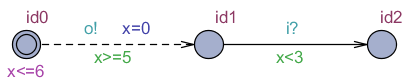
\includegraphics{figures/three-zones.png}};
    \begin{scope}[x={(image.south east)},y={(image.north west)}]
        \node[font=\Large] at (-0.02,0.8) {$\bm{x[0;0 ]}$};
        \node[font=\Large] at (0.06,-0.15) {$\bm{x[0;6]}$};
        \node[font=\Large] at (0.45,0.8) {$\bm{x[0;0 ]}$};
        \node[font=\Large] at (0.28,0) {$\bm{x[5;6 ]}$};
        \node[font=\Large] at (0.5,0) {$\bm{x[0;\infty )}$};
        \node[font=\Large] at (0.7,0) {$\bm{x[0;3 )}$};
        \node[font=\Large] at (0.83,0.8) {$\bm{x[0;3 )}$};
        \node[font=\Large] at (0.92,0) {$\bm{x[0;\infty )}$};
    \end{scope}
\end{tikzpicture}
\caption{Demonstration of arrival, invariant and guard zones} \label{fig:three-zones}
\end{figure}

Zones referred to as \textit{invariant zones} are the ones normally depicted below the location. As a rule, the invariant zone is derived from the arrival zone by performing the delay operation followed by the application of all invariants belonging to the corresponding location. The invariant zone shown under location \textbf{id0} provides information about how long one can stay in the same location by delaying (up to \textbf{6} time units).
 
The last zone to be introduced - \textit{guard zone}, refers to the zone representing all possible clock valuations during which an edge can be taken. The guard zone is derived from the invariant zone by applying all guards associated with that edge. For example, the edge from \textbf{id0} to \textbf{id1} can only be taken with clock \textbf{x} valuations belonging to an interval from \textbf{5} to \textbf{6}.
 
The arrival zone of the target of an edge is then derived from the guard zone of that edge by applying all associated resets. Therefore, the arrival zone at location \textbf{id1} is shaped by the reset on the edge leading to that location, whereas the arrival zone at location \textbf{id2} is equivalent to the guard zone of the edge leading to that location due to the absence of resets.

Even though many of these zones may seem obvious and intuitively derivable from the image of an automaton, in the code of \jecdar these zones are the only source of information during the computation of Refinement, Composition and Conjunction and therefore all of the further algorithms operate with the presented zones.
\chapter{Observations and  inconsistencies}\label{ch:inconst}

This chapter presents observations which were made about various features of \ecdar, including refinement, implementation, consistency and determinism checks. These observations help us to get a better understanding of features that we will implement. We are also going to show the inconsistencies which were found between \textsc{Ecdar} 0.10 and the theory and can be considered as flaws or bugs in the implementation. This is very important as all of the test cases of \jecdar are also tested in \ecdar 0.10, and therefore we must know which test cases we have to treat correctly with respect to theory. We will also explain why these kind of inconsistencies might be happening.

\section{An automaton does not refine itself}\label{sec:selfRef}
Based on the rules mentioned in Section \ref{sec:refRules}, the right side of the refinement has to be able to delay at least as much as the left side or more, which will always be the case in the same automaton, because of guards and invariants being the same. The same holds for outputs and inputs, since identical automata will always be able to comply with the corresponding output or input from the other side. However, if one would investigate \ecdar 0.10 in more depth they would notice that it provides the wrong result in some cases of self refinement. For example the case of Automaton \textbf{C1} from Figure \ref{fig:selfRefinementFail} is one of major inconsistencies of \ecdar 0.10 with the theory. If one would ask \ecdar 0.10 if \textbf{C1} <= \textbf{C1}, it would return that refinement fails. However, according to the theory, self refinement should always hold. If one was to create exactly the same automaton as \textbf{C1}, namely \textbf{C2}, the results would be exactly the same.

Nevertheless, creating the same automaton as \textbf{C1}, except having an additional reset $x=0$ on the input edge as in Figure \ref{fig:selfRefHold} would result in satisfying the refinement. Unfortunately, with the knowledge we have gathered, we cannot explain why \ecdar 0.10 treats it this way.
\begin{figure}
    \centering
    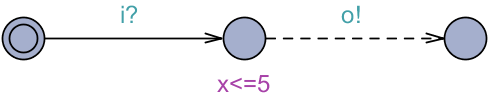
\includegraphics[scale = 0.7]{figures/selfRefFail.png}
    \caption{Automaton C1}
    \label{fig:selfRefinementFail}
\end{figure}

\begin{figure}
    \centering
    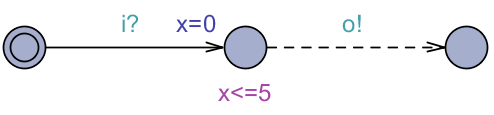
\includegraphics[scale = 0.7]{figures/selfRefHold.png}
    \caption{Automaton C3}
    \label{fig:selfRefHold}
\end{figure}

\section{No Specification as such}\label{sec:specification}
Based on \textcite{David:2010}, there exists a feature called specification, which we have described in \textcite{Jecdar:2019}. Throughout the year we have created multiple examples of specification checks in order to figure out how to properly implement it. However, we could not understand how exactly it works, since \ecdar 2.2 would return results which are completely incorrect according to the theory.

One of the observations that we were able to make when we started using \ecdar 0.10 was that asking for a specification check would return consistency results. We were able to see this only because \ecdar 0.10 returns an answer with a brief explanation, unlike \ecdar 2.2 which only returns true or false. This implies that \ecdar does not grant the possibility of checking for Specification.

Considering the fact that an automaton is a specification if each of its states are input-enabled and we are only working with input-enabled systems, then every automaton is a Specification. Therefore, there is no reason to have the feature Specification check as such.


\section{Partial input-enabledness}\label{sec:input-enabledness}
According to \textcite{David:2010}, "We restrict ourselves to input-enabled systems. This makes it impossible to reach an immediate deadlock state, where a component proposes an output that cannot be captured by the other component". This implies that \ecdar converts each automaton into a corresponding automaton which is input-enabled or treats it as if it was input-enabled. However, in some cases, \ecdar fails to treat an automaton as if it was input-enabled, which makes it inconsistent to the theory. We assume, that \ecdar imagines that there exist a loop of every input in every location, though it never tries to take these self loops first, which cuts out some of the solutions. 

For example, Figure \ref{fig:P4} and Figure \ref{fig:P5} represent two automata, \textbf{P4} and \textbf{P5} respectively and we deal with the case of \textbf{P4} <= \textbf{P5}. Refinement starts in state pair (\textbf{id0}, \textbf{id3}) where it checks if the right side can delay as much as the left side, which is true, then the left side checks if it has any outgoing outputs. Since there are no outputs, the right side checks for inputs, where it finds the input edge \textbf{i?}. Now one has to check if the left side can accept the same input at any given point when the right side is able to. This is true, since the right side can take that input edge at $[3;\infty]$, while the left side can do it at $[0;\infty]$. Then we arrive to the next state pair (\textbf{id0}, \textbf{id3}) with $[3;\infty]$, where we perform the delay check again, and it returns true. After the delay check one has to check for any outgoing outputs from the left side of the refinement, however given the fact that we arrive with the value of clock $y$ being $3$ or above, we are never able to take the \textbf{o!} output edge. The next step is to check if there are any input edges going from the right side and since there are none, the refinement according to \ecdar holds.
\begin{figure}
    \centering
    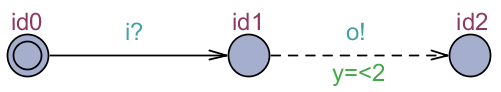
\includegraphics[scale = 0.7]{figures/P4.png}
    \caption{Automaton P4}
    \label{fig:P4}
\end{figure}
\begin{figure}
    \centering
    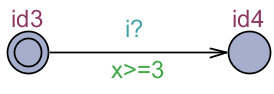
\includegraphics[scale = 0.7]{figures/P5.png}
    \caption{Automaton P5}
    \label{fig:P5}
\end{figure}

However, if one takes into consideration input-enabledness, there would be an additional path in the refinement. Figure \ref{fig:P4InputE} and Figure \ref{fig:P5InputE} provide a view of how \textbf{P4} and \textbf{P5} would look with the addition of input-enabledness. We are again concerned with the same case, \textbf{P4} <= \textbf{P5}, their state space exploration path can be seen at Figure \ref{fig:statePairsP4P5}. After checking for delays in the initial states, one can take a different path and do the self-loop on input \textbf{i?} on the right side, while on the left side taking the same edge as before, ending up in the state pair (\textbf{SP 1}) with the value of clock $x$ being $[0;3)$. Since our arrival time includes values below $2$, one can take the output edge \textbf{o!} on the left side, but the right side cannot comply and the refinement fails.

\begin{figure}
    \centering
    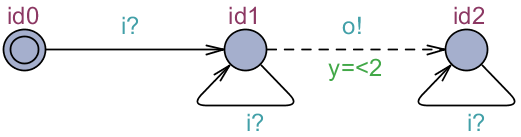
\includegraphics[scale = 0.7]{figures/P4InputEnabled.png}
    \caption{Automaton P4 input-enabled}
    \label{fig:P4InputE}
\end{figure}
\begin{figure}
    \centering
    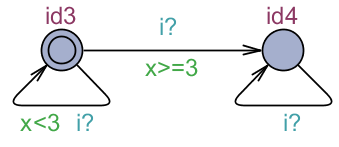
\includegraphics[scale = 0.7]{figures/P5InputEnabled.png}
    \caption{Automaton P5 input-enabled}
    \label{fig:P5InputE}
\end{figure}
\begin{figure}
\centering
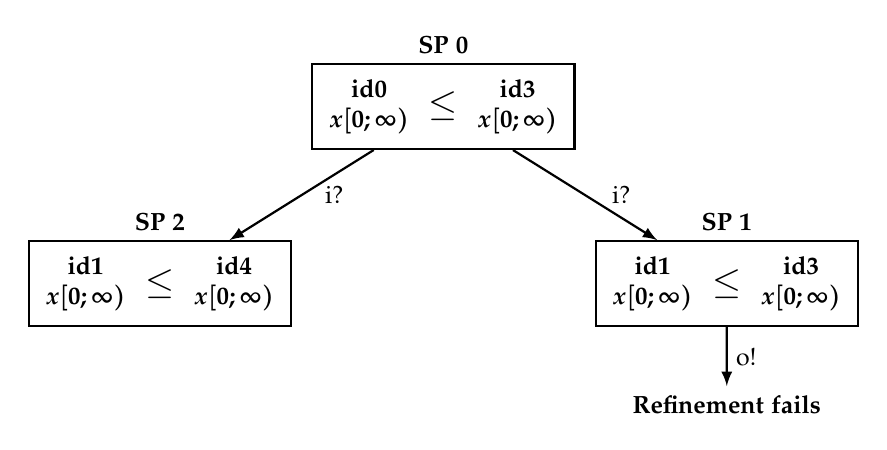
\begin{tikzpicture}[thick,scale=0.9, every node/.style={scale=0.9}]
    \node[draw, anchor=south west,inner sep=0,  minimum width=3.7cm, minimum height=1.2cm] (box) at (0,0) {};
        \begin{scope}[ x={(box.south east)},y={(box.north west)}]
        \node[font=\Large] (a) at (box) {$\leq$};
        \node[align=center, left = 0.1mm of a] {\textbf{id0}\\$\bm{x[0;\infty)}$};
        \node[align=center, right = 0.1mm of a] {\textbf{id3}\\$\bm{x[0;\infty)}$};
        
        \node[align=center, above=0.25cm  of a](k)  {\textbf{SP 0}};
        \end{scope}
        
    \node[draw, anchor=south west,inner sep=0,  minimum width=3.7cm, minimum height=1.2cm] (box1) at (4,-2.5) {};
        \begin{scope}[ x={(box.south east)},y={(box.north west)}]
        \node[font=\Large] (a) at (box1) {$\leq$};
        \node[align=center, left = 0.1mm of a] {\textbf{id1}\\$\bm{x[0;\infty)}$};
        \node[align=center, right = 0.1mm of a] {\textbf{id3}\\$\bm{x[0;\infty)}$};
        \node[align=center, below= 1cm of a](k)  {\textbf{Refinement fails}};
        \draw [-latex,thick] (box1) --  node [right] {o!} (k) ;
        \node[align=center, above=0.25cm  of a](k)  {\textbf{SP 1}};
        \end{scope}
    \node[draw, anchor=south west,inner sep=0,  minimum width=3.7cm, minimum height=1.2cm] (box2) at (-4,-2.5) {};
        \begin{scope}[ x={(box.south east)},y={(box.north west)}]
        \node[font=\Large] (a) at (box2) {$\leq$};
        \node[align=center, left = 0.1mm of a] {\textbf{id1}\\$\bm{x[0;\infty)}$};
        \node[align=center, right = 0.1mm of a] {\textbf{id4}\\$\bm{x[0;\infty)}$};
        
        \node[align=center, above = 0.25cm of a](k)  {\textbf{SP 2}};
        \end{scope}
    \draw [-latex,thick] (box) --  node [right] {\hspace{0.25cm}i?} (box1) ;
    \draw [-latex,thick] (box) --  node [right] {\hspace{0.2cm}i?} (box2) ;

\end{tikzpicture}
\caption{State pairs of $P4<=P5$}
\label{fig:statePairsP4P5}
\end{figure}
To conclude, \ecdar gives the wrong results in cases like the ones mentioned above, since it does not take into consideration input-enabledness, even though it is stated that within this field input-enabledness should be assumed.

\section{Invariant bug}\label{sec:case1}
The case of refinement \textbf{T6} <= \textbf{T5}, whose components are illustrated in Figures \ref{fig:T6} and \ref{fig:T5}, holds according to \ecdar 0.10. In order to understand if this is correct, one has to take a closer look at how refinement works in this case. It starts in the initial states \textbf{id1} and \textbf{id4}, where the delay check is performed with positive results, afterwards the left side outputs with an \textbf{ro!}, while the right is capable of complying to it. The delay check is once again performed on the next state pair (\textbf{id1}, \textbf{id5}) - match. Now the right side is ready to move with input edge \textbf{ri?}, however the left side cannot comply with it, thus the refinement fails.

Surprisingly, if the invariant from location \textbf{id1} or \textbf{id2} (or even both) was removed, then the tool would show that the refinement fails. It is important to remember that according to the theory, in this example the invariants should not make a difference, since the refinement would still fail due to the left side not being able to comply with an input.
\begin{figure}
    \centering
    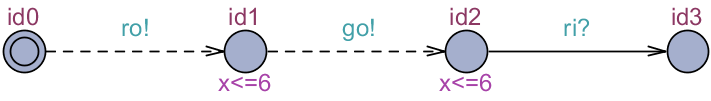
\includegraphics[scale = 0.7]{figures/T6.png}
    \caption{Automaton T6}
    \label{fig:T6}
\end{figure}
\begin{figure}
    \centering
    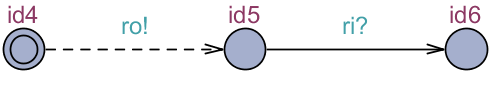
\includegraphics[scale = 0.7]{figures/T5.png}
    \caption{Automaton T5}
    \label{fig:T5}
\end{figure}
\section{Invariant bug nr2}\label{sec:invBug}
An important example in our observations was the refinement (\textbf{T1} || \textbf{T2}) <= \textbf{T3}, as it revealed a similar bug to the one mentioned in Section \ref{sec:case1}. This case is slightly different, since depending on the invariant value or its existence, the result is different. One can see the automata that are participating in this refinement in Figures \ref{fig:T1}, \ref{fig:T2} and \ref{fig:T3}. Figure \ref{fig:statePairsT1T2T3} provides the state space exploration of the refinement check on such automata, according to the theory. Each box provides the view of a state pair in the refinement. Inside the state pair, one can see a simplified version of the zones, which are represented as intervals. The green color marks the value in the interval which forces the remaining zones in the corresponding state pair to shrink. Lastly, the red color indicates places where the other side of the refinement cannot comply to the leading one.
 
\begin{itemize}
    \item (\textbf{State pair 0}) left side can delay up to 300, right side - match. Takes an \textbf{i!} edge.
    \item (\textbf{State pair 1}) left side can delay up to 1, right side - match. Delay check holds and takes \textbf{ri?} edge.
    \item (\textbf{State pair 2}) left side can delay up to 1, right side - match. Takes an \textbf{i!} self loop edge, automaton moves in composition as well with an \textbf{i?}.
    \item (\textbf{State pair 3}) left side can delay up to 1, right side - match. Cannot move anywhere anymore, since on the left side the invariant on \textbf{id2} is $x<=1$ and it blocks the possibility to move, the only output edge has a guard $x>=400$, while the right side does not have any input edges to force a movement.
    \item (\textbf{State pair 0}) left side can delay up to 300, right side - match. Takes an \textbf{ri?} edge - refinement move.
    \item (\textbf{State pair 4}) left side can delay up to 300, right side - 12, fail.
\end{itemize}


\begin{figure}
\centering

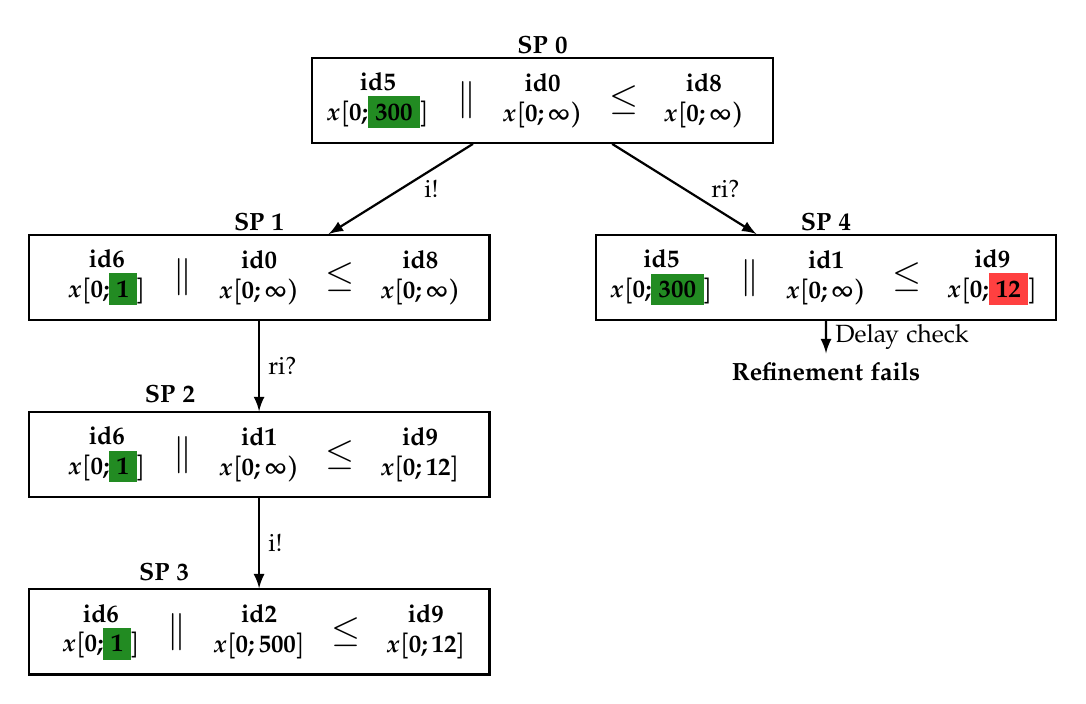
\begin{tikzpicture}[thick,scale=0.9, every node/.style={scale=0.9}]

    
    \node[draw, anchor=south west,inner sep=0,  minimum width=6.5cm, minimum height=1.2cm] (box) at (0,0) {};
        \begin{scope}[ x={(box.south east)},y={(box.north west)}]
        \node[align=center] (a) at (box) {\textbf{id0}\\$\bm{x[0;\infty)}$};
        \node[font=\Large, left = 0.1cm of a] {$\parallel$};
        \node[align=center, left = 0.7cm of a] {\textbf{id5}\\$\bm{x[0;$\colorbox{ForestGreen}{$300$}$]}$};
        \node[font=\Large, right = 0.1cm of a] {$\leq$};
        \node[align=center, right = 0.8cm of a] {\textbf{id8}\\$\bm{x[0;\infty)}$};
        
        \node[align=center, above=0.1mm  of a](k)  {\textbf{SP 0}};
        \end{scope}
        
    \node[draw, anchor=south west,inner sep=0,  minimum width=6.5cm, minimum height=1.2cm] (box1) at (4,-2.5) {};
        \begin{scope}[ x={(box1.south east)},y={(box1.north west)}]
        \node[align=center] (a) at (box1) {\textbf{id1}\\$\bm{x[0;\infty)}$};
        \node[font=\Large, left = 0.1cm of a] {$\parallel$};
        \node[align=center, left = 0.7cm of a] {\textbf{id5}\\$\bm{x[0;$\colorbox{ForestGreen}{$300$}$]}$};
        \node[font=\Large, right = 0.1cm of a] {$\leq$};
        \node[align=center, right = 0.8cm of a] {\textbf{id9}\\$\bm{x[0;$\colorbox{coralred}{$12$}$]}$};
        
        \node[align=center, above=0.1mm  of a](k)  {\textbf{SP 4}};
        \node[align=center, below= 0.5cm of a](k)  {\textbf{Refinement fails}};
        \draw [-latex,thick] (box1) --  node [right] {Delay check} (k) ;
        \end{scope}
    \node[draw, anchor=south west,inner sep=0,  minimum width=6.5cm, minimum height=1.2cm] (box2) at (-4,-2.5) {};
        \begin{scope}[ x={(box.south east)},y={(box.north west)}]
        \node[align=center] (a) at (box2) {\textbf{id0}\\$\bm{x[0;\infty)}$};
        \node[font=\Large, left = 0.1cm of a] {$\parallel$};
        \node[align=center, left = 0.7cm of a] {\textbf{id6}\\$\bm{x[0;$\colorbox{ForestGreen}{$1$}$]}$};
        \node[font=\Large, right = 0.1cm of a] {$\leq$};
        \node[align=center, right = 0.8cm of a] {\textbf{id8}\\$\bm{x[0;\infty)}$};
        \node[align=center, above=0.1mm  of a](k)  {\textbf{SP 1}};
        \end{scope}
    \node[draw, anchor=south west,inner sep=0,  minimum width=6.5cm, minimum height=1.2cm] (box3) at (-4,-5) {};
        \begin{scope}[ x={(box.south east)},y={(box.north west)}]
        \node[align=center] (a) at (box3) {\textbf{id1}\\$\bm{x[0;\infty)}$};
        \node[font=\Large, left = 0.1cm of a] {$\parallel$};
        \node[align=center, left = 0.7cm of a] {\textbf{id6}\\$\bm{x[0;$\colorbox{ForestGreen}{$1$}$]}$};
        \node[font=\Large, right = 0.1cm of a] {$\leq$};
        \node[align=center, right = 0.8cm of a] {\textbf{id9}\\$\bm{x[0;12]}$};
        \node[align=center, above left=0.1cm  of a](k)  {\textbf{SP 2}};
        \end{scope}
    \node[draw, anchor=south west,inner sep=0,  minimum width=6.5cm, minimum height=1.2cm] (box4) at (-4,-7.5) {};
        \begin{scope}[ x={(box.south east)},y={(box.north west)}]
        \node[align=center] (a) at (box4) {\textbf{id2}\\$\bm{x[0;500]}$};
        \node[font=\Large, left = 0.1cm of a] {$\parallel$};
        \node[align=center, left = 0.7cm of a] {\textbf{id6}\\$\bm{x[0;$\colorbox{ForestGreen}{$1$}$]}$};
        \node[font=\Large, right = 0.1cm of a] {$\leq$};
        \node[align=center, right = 0.8cm of a] {\textbf{id9}\\$\bm{x[0;12]}$};
        \node[align=center, above left=0.1cm  of a](k)  {\textbf{SP 3}};
        \end{scope}
    \draw [-latex,thick] (box) --  node [right] {\hspace{0.25cm}ri?} (box1) ;
    \draw [-latex,thick] (box) --  node [right] {\hspace{0.2cm}i!} (box2) ;
    \draw [-latex,thick] (box2) --  node [right] {ri?} (box3) ;
    \draw [-latex,thick] (box3) --  node [right] {i!} (box4) ;
    
\end{tikzpicture}
\caption{State pairs of $T1||T2<=T3$}
\label{fig:statePairsT1T2T3}
\end{figure}
Nevertheless, performing a {refinement} check in \ecdar 0.10 produces a different result, which is inconsistent to the theory, namely that it holds. In order to explain why \ecdar 0.10 ends up having different results, we need to take a look at the transition going from location \textbf{id5} to \textbf{id6}. Having the invariant $x<=1$ on location \textbf{id5} would tighten the invariant on \textbf{id5}, since one could never arrive to \textbf{id6} with values above $1$. Thus the delay check in state pair ((\textbf{id1}, \textbf{id5}), \textbf{id9}) would never fail. It is important to note that this is simply a guess, since we cannot be certain why \ecdar 0.10 treats this case differently than the theory.

Another interesting phenomenon happens when removing the invariant from location \textbf{id5}. According to the theory the results should be the same, since without an invariant it would fail in the same state. However, \ecdar 0.10 outputs a different result, stating that the refinement fails. Unfortunately, we have not derived a proper explanation for why \ecdar 0.10 treats this differently than the case with the invariant, which clearly violates the delay check of the refinement.
\begin{figure}
    \centering
    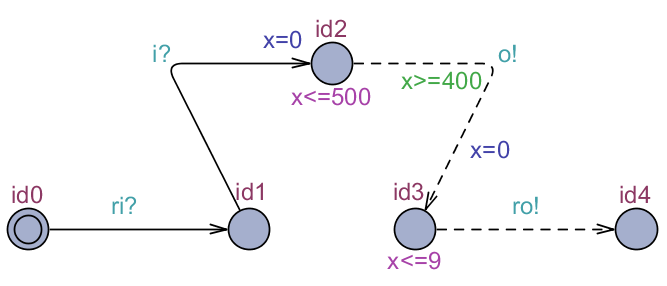
\includegraphics[scale = 0.7]{figures/T1.png}
    \caption{Automaton T1}
    \label{fig:T1}
\end{figure}
\begin{figure}
    \centering
    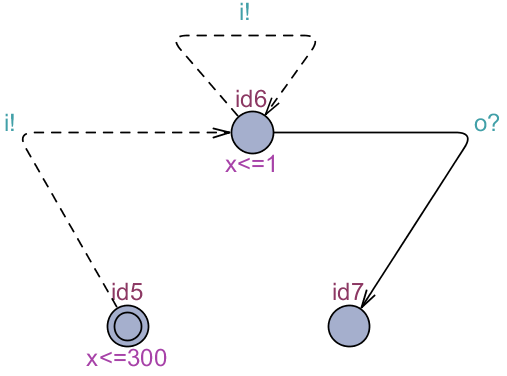
\includegraphics[scale = 0.7]{figures/T2.png}
    \caption{Automaton T2}
    \label{fig:T2}
\end{figure}
\begin{figure}
    \centering
    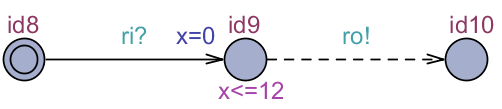
\includegraphics[scale = 0.7]{figures/T3.png}
    \caption{Automaton T3}
    \label{fig:T3}
\end{figure}
\section{Signature check}\label{sec:signatureCheck}
We have observed that \ecdar performs some sort of signature check. Having additional outputs on the left side, while the right side has them only in the signature but not in the component itself breaks the refinement. The same applies for the inputs, having an additional input on the right side, while the left side does not have it even in the signature, the refinement holds. On the other hand, if one would add such an input to the signature, the refinement would fail. The refinement of \textbf{N3<=N4}, whose components can be seen in Figures \ref{fig:N3} and \ref{fig:N4} shows the case where, according to \ecdar, having an input only in the signature of the automaton which is present on the right side leads to the failure of the refinement. However, according to the theory, all the components are input-enabled, which implies that the left side should be able to perform the "imaginary self loop" on the missing input \textbf{i2?}. 

\begin{figure}
    \centering
    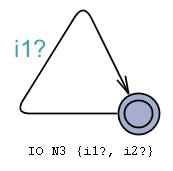
\includegraphics[scale = 0.7]{figures/N3.png}
    \caption{Automaton N3}
    \label{fig:N3}
\end{figure}
\begin{figure}
    \centering
    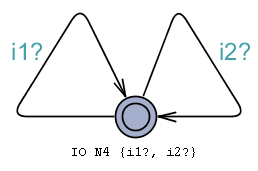
\includegraphics[scale = 0.7]{figures/N4.png}
    \caption{Automaton N4}
    \label{fig:N4}
\end{figure}

\section{Types of consistency check}\label{sec:minConsistency}
In the beginning we were only aware of the existence of one type of consistency, which needs to check the whole automaton in order to make sure it is consistent. However, throughout our project an observation have been made, that there exist different types of consistencies: 
\begin{itemize}
    \item Least fixpoint consistency
    \item Greatest fixpoint consistency
    \item Full consistency
\end{itemize}
This semester we are only going to handle the least fixpoint and the full consistency. The full consistency has to check the whole automaton in order for it to return a result. On the other hand, the least fixpoint consistency can prune some of the edges in order to find the smallest part of the automaton that is consistent. It can prune all the outputs, since they are controllable, unlike inputs which can neither be controlled nor pruned. Opposite to least fixpoint consistency, the greatest fixpoint consistency finds the biggest part of an automaton, which is consistent.

\ecdar provides only one type of consistency - the least fixpoint consistency check. Consider the example in Figure \ref{fig:G21}, which starts in the initial location, where there is an output edge going from it. Since it is an output, we can prune the rest of the automaton and have the least fixpoint consistency. On location \textbf{id2} there is an invariant and there are no output edges going from it that could solve the problem. However, since the rest of the automaton was pruned, this does not matter anymore.
\begin{figure}
    \centering
    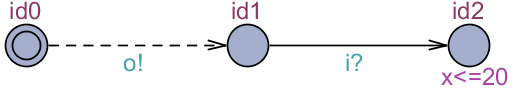
\includegraphics[scale = 0.7]{figures/G21.png}
    \caption{Automaton G21}
    \label{fig:G21}
\end{figure}

\section{Determinism bug}\label{sec:determBug}
An important aspect to remember is that all automata must be deterministic. If there are multiple outgoing edges from the same location with the same action, a determinism check has to be made in order to ensure that there exists only one path at any given point in time. \ecdar always performs a determinism check before running queries and it appears as though it is always able to determine correctly if an automaton is deterministic.

In spite of this, we have succeeded to find a case where \ecdar fails at the determinism check. Consider Figure \ref{fig:P8}, where \ecdar states that this automaton is deterministic. In this example there are three different edges from the initial location \textbf{id0}. In the case of the two edges that lead to location \textbf{id2}, the intervals in which these edges can be traversed do not overlap, but in the case of the third edge which leads to location \textbf{id1}, the interval overlaps with one of the other edges. Thus, the determinism check should fail. It seems like in the cases where there are multiple edges going from one location to another one, they are being excluded from further determinism checks in \ecdar.
\begin{figure}
    \centering
    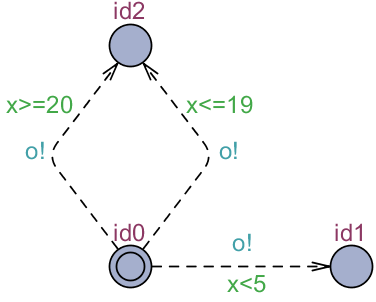
\includegraphics[scale = 0.7]{figures/P8.png}
    \caption{Automaton P8}
    \label{fig:P8}
\end{figure}
\section{Global time correspondence}\label{sec:globalTime}
Another important observation that was made was about \ecdar's global time correspondence. Dealing with time in this field is important, so it is crucial to understand as much as possible about it. One has to keep in mind that arriving at a certain time in two automata that are in a refinement relation will always result in being at the same time in accordance with its minimum and maximum values.

In order to understand this better, one should take a look at the relation of \textbf{K5} <= \textbf{K6}, which is represented in Figures \ref{fig:K5} and \ref{fig:K6}. The arrival time in \textbf{id1} is $0$, because of the reset and the arrival time in \textbf{id4} is $5$. The time correspondence is simple in this case, since in both automata we have only one value. However, in the case of the arrival times in \textbf{id2} and in \textbf{id5}, they will end up being intervals, $[0;10]$ and $[5;15]$, respectively. The actual arrival time in the previously mentioned state pair would be somewhere in the middle, but at the same point in time, given the minimum or maximum values of each interval. It is impossible to arrive in such a state pair with one of the automata being at its maximum arrival time and the other one at its minimum. The reasoning behind this is that time always moves at the same rate and it cannot be frozen in any of the automata.
\begin{figure}
    \centering
    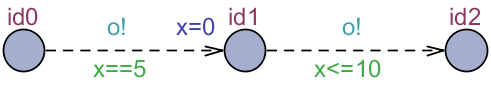
\includegraphics[scale = 0.7]{figures/K5.png}
    \caption{Automaton K5}
    \label{fig:K5}
\end{figure}
\begin{figure}
    \centering
    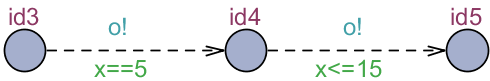
\includegraphics[scale = 0.7]{figures/K6.png}
    \caption{Automaton K6}
    \label{fig:K6}
\end{figure}


\section{Exploration of refinement with input-enabledness}\label{sec:case2}
After analysing the refinement of \textbf{T9} <= \textbf{T8}, which is illustrated in Figures \ref{fig:T8} and \ref{fig:T9}, valuable information of how refinement works in \ecdar can be derived. It starts in the initial locations \textbf{id4} and \textbf{id0}, where the delay check is satisfied. Afterwards, the right side makes a move on input edge \textbf{i1?}, while the left side is able to comply. Now the left side has only one move, which is a common input \textbf{i2?}, while the left side also has one move, namely common output \textbf{o!}. Here the refinement check is complete and \ecdar returns true, which implies that the rest of the automaton is not explored, since refinement would fail at a later point.
\begin{figure}
    \centering
    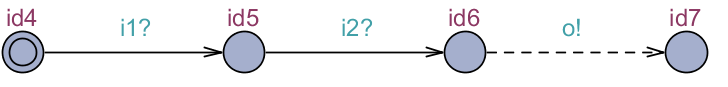
\includegraphics[scale = 0.7]{figures/T9.png}
    \caption{Automaton T9}
    \label{fig:T9}
\end{figure}
\begin{figure}
    \centering
    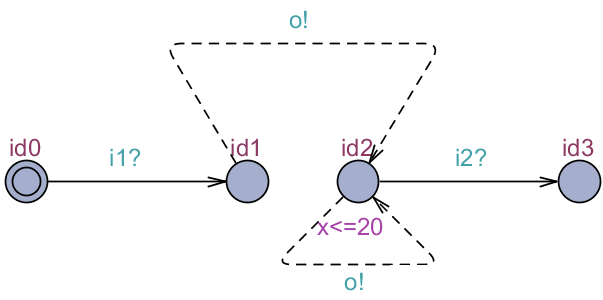
\includegraphics[scale = 0.7]{figures/T8.png}
    \caption{Automaton T8}
    \label{fig:T8}
\end{figure}
According to the rules of refinement, the left side can force to move on outputs and the right side can do the same on inputs. The fact that \ecdar stops the exploration at this point is in accordance with the theory, since it is not stated what happens when the only possible movements are with the input from the left and with the output from the right. However, if we take into consideration input-enabledness, everything changes. Now, according to the theory the refinement should fail. The state space exploration is provided in Figure \ref{fig:statePairsT9T8}, which is performed in accordance to the theory.

The refinement check begins in state pair 0, where the right side can comply to the delay check. Both sides move with an input edge \textbf{i1?}. In state pair 1 the delays match and now we may perform a self loop on location \textbf{id1} on input \textbf{i2?}, while the left side can comply to it. Now the left side is the leading one with an output edge \textbf{o!}, which can be traversed with $\bm{x\in[0;\infty]}$, while the right side cannot comply to it, since its output edge \textbf{o!} can be traversed only with $\bm{x\in[0;20]}$, thus the refinement fails.

\begin{figure}
\centering
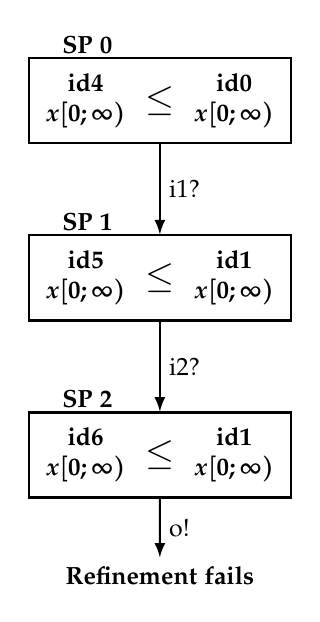
\begin{tikzpicture}[thick,scale=0.9, every node/.style={scale=0.9}]
    \node[draw, anchor=south west,inner sep=0,  minimum width=3.7cm, minimum height=1.2cm] (box) at (0,0) {};
        \begin{scope}[ x={(box.south east)},y={(box.north west)}]
        \node[font=\Large] (a) at (box) {$\leq$};
        \node[align=center, left = 0.1mm of a] {\textbf{id4}\\$\bm{x[0;\infty)}$};
        \node[align=center, right = 0.1mm of a] {\textbf{id0}\\$\bm{x[0;\infty)}$};
        
        \node[align=center, above left=0.25cm  of a](k)  {\textbf{SP 0}};
        \end{scope}
        
    \node[draw, anchor=south west,inner sep=0,  minimum width=3.7cm, minimum height=1.2cm] (box1) at (0,-2.5) {};
        \begin{scope}[ x={(box.south east)},y={(box.north west)}]
        \node[font=\Large] (a) at (box1) {$\leq$};
        \node[align=center, left = 0.1mm of a] {\textbf{id5}\\$\bm{x[0;\infty)}$};
        \node[align=center, right = 0.1mm of a] {\textbf{id1}\\$\bm{x[0;\infty)}$};
        
        \node[align=center, above left=0.25cm  of a](k)  {\textbf{SP 1}};
        \end{scope}
    \node[draw, anchor=south west,inner sep=0,  minimum width=3.7cm, minimum height=1.2cm] (box2) at (0,-5) {};
        \begin{scope}[ x={(box.south east)},y={(box.north west)}]
        \node[font=\Large] (a) at (box2) {$\leq$};
        \node[align=center, left = 0.1mm of a] {\textbf{id6}\\$\bm{x[0;\infty)}$};
        \node[align=center, right = 0.1mm of a] {\textbf{id1}\\$\bm{x[0;\infty)}$};
        
        \node[align=center, above left=0.25cm  of a](k)  {\textbf{SP 2}};
        \node[align=center, below= 1cm of a](k)  {\textbf{Refinement fails}};
        \draw [-latex,thick] (box2) --  node [right] {o!} (k) ;
        \end{scope}

    \draw [-latex,thick] (box) --  node [right] {i1?} (box1) ;
    \draw [-latex,thick] (box1) --  node [right] {i2?} (box2) ;
\end{tikzpicture}
\caption{State pairs of $T9<=T8$}
\label{fig:statePairsT9T8}
\end{figure}


\section{Treatment of syncs as outputs}\label{sec:case3}
The refinement which is illustrated in Figure \ref{fig:P8||P9<=P10} holds in \ecdar. However, according to the theory, in this case it should not even pass the signature check. The reasoning behind this is that the left side cannot have an action \textbf{i} being an input and an output at the same time, while on the left it exists as an input. If on the right side \textbf{i} would be an output  instead of an input, then the refinement would hold. This happens because syncs are treated as outputs, therefore \textbf{i} would be an output on both sides and the signature check would pass.
\begin{figure}
\centering
\begin{tikzpicture}[thick,scale=0.7, every node/.style={scale=0.7}]
    \node[anchor=south west,inner sep=0] (image) at (0,0)
    {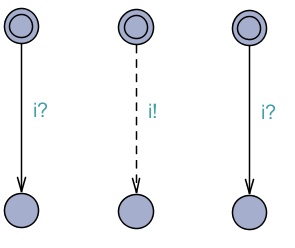
\includegraphics{figures/P8CompP9RefP10.png}};
    \begin{scope}[x={(image.south east)},y={(image.north west)}]
        
        \node[font=\Large] at (0.65,0.5) {$\Scale[2]{{\leq}}$};
        \node[font=\Large] at (0.27,0.5) {$\Scale[2]{{\parallel}}$};
    \end{scope}
\end{tikzpicture}
\caption{Refinement which should not pass the signature check} \label{fig:P8||P9<=P10}
\end{figure}
\chapter{Practical Concepts} \label{ch:concepts}
This chapter presents practical concepts, which were introduced in order to solve the refinement issues in \jecdar. Not all of the considered concepts have proven to be correct or suitable, such as concepts of arrival zone, min/max, accumulative delays and timeline. We show the problems these concepts were meant to solve and flaws of each of them. Finally we present the concept of a global zone which is the one currently used in \jecdar.

\section{Zone unions} \label{sec:zoneUnions}

The data structure that we use for representing clock constraints, the DBM, is very powerful and efficient for our purposes. Until now, the operations that we needed to perform on zones(e.g., apply constraint, delay, intersection) did not cause any issues.

A problem arose when we discovered the need to add multiple zones together in order to see "the full zone" for which a certain action is enabled. DBMs "have a well-known shortcoming: they are not closed under set-union. This comes from the fact that a set represented by a DBM is convex, while the union of two convex sets is not necessarily convex", as explained in \textcite{UppaalSecrets}.

This means that if we must perform addition or subtraction on DBMs, we must find a different data structure to store the result. The most logical approach, if we are to keep using DBMs, is to introduce the concept of zone union. On top of this, the DBM library provides support for zone unions, which simplifies the task for us.

\textcite{UppaalSecrets} also mentions that with a different data structure for zones, namely CDDs (Clock Difference Diagrams), performing operations such as addition or subtraction of zones would not be a problem, as these are closed under set-union. In spite of this, as long is there is no library support for CDDs, it is more convenient for us to continue using DBMs.

\section{Absolute zone}
The very first big concept that has been introduced in the project is \textit{absolute zone}. The concept was summoned to solve a number of problems related to the verification of the availability of an edge in the context of one or more automata trying to move simultaneously to a new state in case of refinement and other features. Further we list issues that were meant to be solved by an absolute zone:
\begin{itemize}
    \item Edge availability in an individual automaton given two or more clocks that are constrained such that an edge cannot be taken.
    \item Edge availability given that the constrained clocks (at least two) might end up having greatly differing possible valuations at some point of the state space exploration. 
    \item Transition (number of edges) availability in the case of two or more automata performing a simultaneous move in such features as Refinement, Composition and Conjunction.
    \item Adjustment of resulting arrival zones given that two or more automata move simultaneously, resulting in arrival zones having to be constrained according to the rules of Refinement, Composition and Conjunction.
\end{itemize}

Generally, an absolute zone should be used during the call to the \textsc{GetNextTransitions()} method described in \textcite{Jecdar:2019}, which returns transitions with all the possible moves from one state to another for an arbitrary amount of automata. It is also important to state that unlike arrival, invariant or guard zone, an absolute zone is not meant to be stored, but rather helps to properly manage the rest of the zones when taking an edge.

\subsection{Examples}
To be able to understand some of the issues better, consider the automaton in Figure \ref{fig:az-first}. Due to the fact that \textbf{id0} is an initial location, the arrival zones state that both of the clocks \textbf{x} and \textbf{y} begin from the value \textbf{0}. In such a scenario an output edge leading to location \textbf{id1} cannot be taken because of the non-intersecting guards for clocks with identical arrival zones. However, constraining the invariant zone with the guards would result in a completely valid zone (shown to the right of the automaton), tricking one into believing that the edge can be traversed.

\begin{figure}
\centering
\begin{tikzpicture}[thick,scale=0.9, every node/.style={scale=0.9}, baseline=0.5cm]
    \node[anchor=south west,inner sep=0] (image) at (0,0)
    {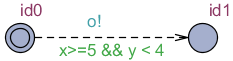
\includegraphics{figures/az-first.png}};
    \begin{scope}[x={(image.south east)},y={(image.north west)}]
        \node[font=\Large] at (-0.05,1.2) {$\bm{x[0;0 ]}$};
        \node[font=\Large] at (-0.05,0.8) {$\bm{y[0;0 ]}$};
        \node[font=\Large] at (0,-0.15) {$\bm{x[0;\infty )}$};
        \node[font=\Large] at (0,-0.55) {$\bm{y[0;\infty )}$};
        \node[font=\Large] at (0.45,-0.2) {$\bm{x[5;\infty )}$};
        \node[font=\Large] at (0.45,-0.6) {$\bm{y[0;4 )}$};
    \end{scope}
\end{tikzpicture} \hspace{1cm}
\begin{tabular}{c|c|c}
        $\leq 0$ & $\leq -5$ & $\leq 0$ \\
        \hline
        $\leq \infty$ & $\leq 0$ & $\leq \infty$ \\
        \hline
        $< 4$ & $< -1$ & $\leq 0$\\
   \end{tabular}
\caption{Unavailable edge in a single automaton and a corresponding valid guard zone} \label{fig:az-first}
\end{figure}

Next, consider a more complex refinement example of two automata excerpts in Figure \ref{fig:az-ref}, where the automaton on the left is challenged to refine the one on the right starting from locations \textbf{id0} and \textbf{id2}. The arrival zones of the two mentioned locations appear to differ to such a significant extent where it might seem from the first glance that the refinement output rule would not hold. 

\begin{figure}
\centering
\begin{tikzpicture}[thick,scale=0.9, every node/.style={scale=0.9}]
    \node[anchor=south west,inner sep=0] (image) at (0,0)
    {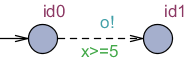
\includegraphics{figures/az-second.png}};
    \begin{scope}[x={(image.south east)},y={(image.north west)}]
        \node[font=\Large] at (-0.05,0.8) {$\bm{x[0;0 ]}$};
        \node[font=\Large] at (0,-0.15) {$\bm{x[0;\infty )}$};
        \node[font=\Large] at (0.5,-0.2) {$\bm{x[5;\infty )}$};
        \node[font=\Large] at (0.68,0.9) {$\bm{x[5;\infty )}$};
        
        \node at (2,0.45) {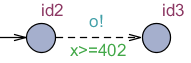
\includegraphics{figures/az-third.png}};
        \node[font=\Large] at (1.45,0.8) {$\bm{x[400;400]}$};
        \node[font=\Large] at (1.5,-0.15) {$\bm{x[400;\infty )}$};
        \node[font=\Large] at (2,-0.2) {$\bm{x[402;\infty )}$};
        \node[font=\Large] at (2.2,1.1) {$\bm{x[405;\infty )}$};
    \end{scope}
\end{tikzpicture}
\caption{Abstract example of an available transition where left automaton refines right automaton} \label{fig:az-ref}
\end{figure}

However, we will discover that the refinement output rule holds in this example. It is explained as follows; the automaton on the left must wait at least \textbf{5} time units before being able to issue an output, whereas the automaton on the right can always follow due to it being able to issue an output after delaying for at least two time units. Additionally, the arrival zone of the second automaton in \textbf{id3} must be adjusted to reflect that an edge was traversed only after delaying for at least \textbf{5} time units, since the right side of the refinement only follows the left side.

\begin{figure}
\centering
\begin{tabular}{c|c}
        $\leq 0$ & $\leq -5$  \\
        \hline
        $\leq \infty$ & $\leq 0$ \\
\end{tabular}
\hspace{2cm}
\begin{tabular}{c|c}
        $\leq 0$ & $\leq -2$  \\
        \hline
        $\leq \infty$ & $\leq 0$ \\
\end{tabular}
\caption{Absolute zones for automata from Figure \ref{fig:az-ref}} \label{fig:az-ref-zones}
\end{figure}

Figure \ref{fig:az-ref-zones} demonstrates two absolute zones that were built for the automata from the example in Figure \ref{fig:az-ref}. The key difference between the absolute zone and such zones as arrival, invariant or guard one, is its independence from the potentially fluctuating values of the arrival zone. The absolute zone is read as follows: the lower bound of a clock states the minimum amount of delay that is necessary to take before the edge becomes available. At least two time units must pass in order to be able to take an edge from location \textbf{id2} to \textbf{id3}, exactly which is reflected in the lower bound of the corresponding absolute zone. 

Oppositely, the upper bound of the clock in the absolute zone states the maximum possible delay that can be done while the edge still remains available. 


\subsection{Implementation details}
Now that we have seen some examples of the issues that the absolute zone is hoped to solve, we will take a look at the algorithm used to compute absolute zones. The function in Algorithm \ref{alg:absolute-zone} demonstrates the main logic used to calculate absolute zones given an invariant zone and the guards of an edge that is challenged for availability.

\begin{algorithm}
\caption{Algorithm to compute absolute zones}
\label{alg:absolute-zone}
\begin{algorithmic}[1]
\Function{getAbsoluteZone}{$invZone, guards$}
\State $absZone \gets invariantZone$
\ForAll{$guard$ in $guards$}
\State $constraint \gets \textsc{BoundToRaw}(guard.value)$
\State $clockLB \gets invZone.clockLB$
\State $clockUB \gets invZone.clockUB$
\If{(firstVisit)}
\State $absZone.\textsc{FreeDown}(guard.clock)$
\EndIf
	\If{($guard \in \{<,\leq \}$)}
        \If{($constraint > clockUB \And clockUB \neq \infty$)}
	        \State $NewUB \gets \textsc{addRawRaw}(clockUB, clockLB)$
	    \Else
	        \State $NewUB \gets \textsc{addRawRaw}(constraint, clockLB)$
	    \EndIf
	    \State $absZone.\textsc{ContstrainDBM(NewUB)}$
	\EndIf
		
	\If{($guard \in \{>,\geq \}$)}
	    \If{($constraint - clockLB < 0$)}
	        \State $NewLB \gets 0$
	    \Else
	        \State $NewLB \gets \textsc{addRawRaw}(constraint, clockLB)$
	    \EndIf
	     \State $absZone.\textsc{ContstrainDBM(NewLB)}$
	\EndIf
\EndFor
\ForAll{$clock$ in $unmodifiedClocks$}
\State $clockLB \gets invZone.clockLB$
\State $clockUB \gets invZone.clockUB$
\If{($clockLB \neq 1$)}
    \State $absZone.\textsc{FreeDown}(clock)$
\EndIf
\If{($clockUB \neq \infty$)}
\State $newUB \gets \textsc{addRawRaw}(clockUB, clockLB)$
\EndIf
\State $absZone.\textsc{ContstrainDBM(NewUB)}$
\EndFor
\State
\State \textbf{return $absZone$}	
\EndFunction
\end{algorithmic}
\end{algorithm}

Overall, the intent is to consider and treat respectively three cases of guards: guards that define the upper bound of the clock (Line 9), guards that define the lower bound of the clock (Line 15) and the absence of guards for certain clocks as such (Line 21). The first two cases related to different guards are treated in the first \textit{for all} loop (Lines 3-20), which is then followed by necessary changes to the bounds of the clocks that had no guards associated with them (Lines 21-28).

First of all, we assign three variables that are essential for further computations - \textit{constraint, clockUB} and \textit{clockLB} (Lines 4-6). Note that these variables are all of type \textbf{raw\_t} and correspond to the DBM library encoded constraints explained in Section \ref{sec:raw-values}. The \textsc{BoundToRaw()} method is used to encode the bounds of the guard into the required encoded constraint.

Due to the fact that constraining any bound of the clock will change the zone only if the applied constraint would tighten the zone, it is necessary to reset the lower bound of the clock that the guard is associated with, but only when that specific clock is handled for the first time (Lines 7-8).

Furthermore, depending on the type of the inequality symbol of the guard, the corresponding bound (upper bound or lower bound) must be calculated and then used to constrain the clock (Lines 10-14 and 16-20). Similarly, for clocks that were not constrained by any of the guards, a lower bound of the resulting zone's clock is freed, whereas its upper bound becomes the difference between the upper and lower bounds of the clock. 

The reason the difference is computed with the help of the \textsc{AddRawRaw()} DBM method is the handy fact that the lower bound constraints result in being encoded as negative raw values. Therefore, the addition of positive $clockUB$ and negative $clockLB$ in Lines 13, 19 and 27 will yield the correct result.

\subsection{Application of absolute zone}
The information contained in the generated absolute zone helps to solve the issues described above. Regardless of the values of the arrival zone and other zones derived from it, we now possess "absolute" information about the time intervals when an edge can be traversed. 

In the case of refinement it becomes a trivial task to check if one side of the refinement is able to follow the other one. To do so, one must compute the highest minimum delay value and the smallest maximum delay value among all clocks. The two resulting \textit{min} and \textit{max} values will represent the minimum delay and the maximum delay that can be taken among all clocks. After the computation is done for both sides of the refinement, it suffices to check the following two conditions:
\begin{itemize}
    \item $min_l \geq min_r$\\
    Check if an edge becomes available on the right side of the refinement earlier or at the same time as on the left side
    \item $max_l \leq max_r$\\
    Check if an edge remains available on the right side for at least as long as on the left side
\end{itemize}

\subsection{Absolute zone issues}
As we will discover later on, the concept of the absolute zone appears to have certain flaws and blind spots.

First of all, historically, the concept of absolute zones appeared and was implemented before the strictness fix, described in Section \ref{sec:strictnessFix}. This means that any addition or subtraction of constraints was a primitive operation due to constant "weak" strictness. From math we know that the addition and subtraction of weak constraints always results in a weak constraint. Due to this fact, the algorithm of the absolute zone did not encounter any issues in its frequently occurring addition or subtraction operations on raw values.

However, together with the strictness fix new problems arose. One of the issues expected to be solved, namely the adjustment of the resulting arrival zones, became impossible to perform correctly without losing or adding solutions to the zones, neither of which are acceptable in terms of correctness. 

\medskip

Moreover, absolute zones do not infer any information from arrival zones and therefore a lot of vital information is lost in the process. Consider the example in Figure \ref{fig:az-identical} where the upper automaton is challenged to refine the bottom one. It is also shown that both invariant and guard zones are absolutely identical in both cases. This means that the algorithm would produce identical absolute zones and naturally, after comparing the resulting \textit{min} and \textit{max} values, we deduce that the refinement holds. 

However, that is not the case in this example! It is easy to show that the refinement cannot hold due to the violation of the refinement output rule, which is caused by the only difference between the two automata - the reset on the edge from \textbf{id0} to \textbf{id1}. Consider having delayed \textbf{250} at location \textbf{id0} and outputting afterwards, resulting at \textit{id1}. The second automaton then follows according to the refinement output rule and gets to \textbf{id4}. Due to the above-mentioned reset, the upper automaton is able to delay up to \textbf{500} time units and output, whereas the bottom one, having arrived with the clock value of \textbf{250} already, will not be able to comply to the left side of the refinement.

Therefore, the concept of the absolute zone alone is not enough to handle all rules of refinement correctly.

\begin{figure}
\centering
\begin{tikzpicture}[thick,scale=0.9, every node/.style={scale=0.9}]
    \node[anchor=south west,inner sep=0] (image) at (0,0)
    {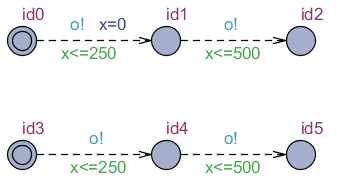
\includegraphics{figures/az-identical.png}};
    \begin{scope}[x={(image.south east)},y={(image.north west)}]
        
        \node[font=\Large] at (0.4,1) {$\bm{x[0;0]}$};
        \node[font=\Large] at (0.48,0.6) {$\bm{x[0;\infty )}$};
        \node[font=\Large] at (0.7,0.6) {$\bm{x[0;500]}$};
        
        \node[font=\Large] at (0.38,0.34) {$\bm{x[0;250]}$};
        \node[font=\Large] at (0.48,-0.05) {$\bm{x[0;\infty )}$};
        \node[font=\Large] at (0.7,-0.05) {$\bm{x[0;500]}$};
    \end{scope}
\end{tikzpicture}
\caption{The refinement of two almost identical automata that does not hold. Upper automaton refines bottom one.} \label{fig:az-identical}
\end{figure}

\section{Concept of Min/Max and zone union subtraction}
After realizing the failure of absolute zones to solve all the issues in the refinement relation, a new idea arose, namely Min/Max. This concept would take into consideration the very minimum of the arrival zone as well as its maximum and compare them to the corresponding guard interval. This comparison is vital when we have a reset on one of the automata, since it shows if both of the automata can delay the same amount before taking a corresponding edge.

Equation \ref{eq:lrMinMax} shows the algorithm which calculates the final min and max values for the left and the right side. In this algorithm $lf$ stands for the left side final values and $rf$ for the right side final values, while $g$ and $a$ stands for guard and arrival zone respectively. After receiving the final min and max values for both of the sides, one has to perform a comparison between them in order to see if both of the sides can traverse an edge at any given value within their intervals. This comparison can be seen in Equation \ref{eq:comparison}.
\begin{multline}
\label{eq:lrMinMax}
\\
lfMin = gMin - aMax\\
lfMax = gMax - aMin\\
rfMin = gMin - aMin\\
rfMax = gMax - aMax\\
\end{multline}
\begin{multline}
\label{eq:comparison}
\\
lfMin \geq rfMin\\
lfMax \leq rfMax\\
\end{multline}
\subsection{Examples of Min/Max}
In order to better understand how the Min/Max algorithm works, it is helpful to look at a few examples. The previously mentioned refinement relation from Figure \ref{fig:az-identical} using absolute zones fails, so this case has to be solved using the Min/Max algorithm mentioned in Equation \ref{eq:lrMinMax}. We are interested in locations, right before the reset happens, namely \textbf{id1} and \textbf{id4}. After the calculations of the final values, which are shown in \ref{eq:calcK3K4}, one can see that one of the rules is not satisfied, thus the refinement does not hold.
\begin{multline}
\label{eq:calcK3K4}
\\
lfMin = 0 - 0 = 0\\
lfMax = 500 - 0 = 500\\
rfMin = 0 - 0 = 0\\
rfMax = 250 - 0 = 250\\
0 \geq 0 \\
500 \rlap{\kern.45em$|$}\leq 250 \\
\end{multline}

To ensure that the algorithm works correctly, one has to take a look at an example which is opposite to the previous one. Figure \ref{fig:K1K2} shows a refinement relation between two automata, the upper one refining the lower one. Imagine a scenario where one would delay at location \textbf{id0} until $x=500$ and then traverse the edge. The arrival value of \textbf{id1} would be $500$, while in location \textbf{id4} - $0$, due to the reset. This would break the refinement relation, since the upper automaton would be able to traverse the output edge \textbf{o!}, while the right side of refinement would not be able to follow, since it has to delay at least $250$ in order to traverse the corresponding edge.

\begin{figure}
\centering
\begin{tikzpicture}[thick,scale=0.9, every node/.style={scale=0.9}]
    \node[anchor=south west,inner sep=0] (image) at (0,0)
    {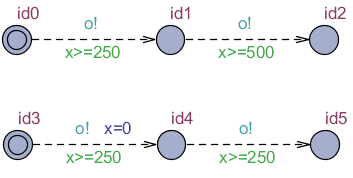
\includegraphics{figures/K1K2.png}};
    \begin{scope}[x={(image.south east)},y={(image.north west)}]
        
        \node[font=\Large] at (0.37,1) {$\bm{x[250;\infty)}$};
        \node[font=\Large] at (0.48,0.6) {$\bm{x[0;\infty )}$};
        \node[font=\Large] at (0.7,0.6) {$\bm{x[500;\infty)}$};
        
        \node[font=\Large] at (0.4,0.38) {$\bm{x[0;0]}$};
        \node[font=\Large] at (0.48,0.02) {$\bm{x[0;\infty )}$};
        \node[font=\Large] at (0.7,0) {$\bm{x[250;\infty)}$};
    \end{scope}
\end{tikzpicture}
\caption{The refinement of two almost identical automata that does not hold. Upper automaton refines bottom one.} \label{fig:K1K2}
\end{figure}
Knowing that the refinement relation does not hold, one can check if the Min/Max algorithm would provide the same results. Once again we must look at the location that has a reset preceding it. The calculation of Min/Max from locations \textbf{id1} and \textbf{id4} can be seen in Figure \ref{eq:calcK1K2}. The rule, which requires $lfMin \geq rfMin$ does not hold, thus the Min/Max algorithm provides the same results.
\begin{multline}
\label{eq:calcK1K2}
\\
lfMin = 500 - \infty = 0\\
lfMax = \infty - 250 = \infty\\
rfMin = 250 - 0 = 250\\
rfMax = \infty - 0 = \infty\\
0 \rlap{\kern.45em$|$}\geq 250 \\
\infty \leq \infty \\
\end{multline}

\subsection{Issues of Min/Max}
This algorithm solves all the problems where there is only one outgoing edge from each of the locations. However, when we start taking into consideration examples such as in Figure \ref{fig:H1H2}, where the automaton has more than one outgoing edge, the algorithm starts providing incorrect results. The exact scenario is when the left automaton refines the right one. Both of the edges on the right side combined are capable of covering output \textbf{o!} at any given point where the left side would output, thus the refinement holds in this case. However, if one would try to place the values into the Min/Max formula, it would break. Consequently, we need a new approach for dealing with multiple outgoing edges.

\begin{figure}
\centering
\begin{tikzpicture}[thick,scale=0.9, every node/.style={scale=0.9}]
    \node[anchor=south west,inner sep=0] (image) at (0,0)
    {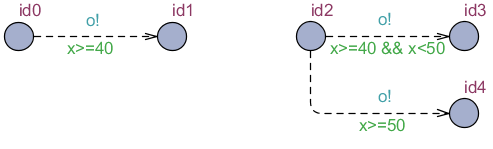
\includegraphics{figures/H1H2.png}};
    \begin{scope}[x={(image.south east)},y={(image.north west)}]
        
        \node[font=\Large] at (-0.02,0.93) {$\bm{x[0;0]}$};
        \node[font=\Large] at (0.03,0.56) {$\bm{x[0;\infty )}$};
        \node[font=\Large] at (0.2,0.56) {$\bm{x[40;\infty)}$};
        
        \node[font=\Large] at (0.57,0.93) {$\bm{x[0;0]}$};
        \node[font=\Large] at (0.78,0.55) {$\bm{x[40;50 )}$};
        \node[font=\Large] at (0.78,0.03) {$\bm{x[50;\infty)}$};
    \end{scope}
\end{tikzpicture}
\caption{Multiple outgoing edges from a single location} \label{fig:H1H2}
\end{figure}

Previously in Section \ref{sec:zoneUnions}, we have discovered the existence of DBM unions which are called Federations. When working with Federations, the subtraction method can be used in order to check if one of the Federations does not cover some part of the zone. Using this new approach one can easily deal with covering the zones of multiple edges. With this newly obtained knowledge, we have improved the Min/Max algorithm to use subtraction of federations and slightly modified some of the formulas, which can be seen in Equation \ref{eq:newMinMax}. The new Min/Max algorithm made it possible to verify if the refinement relation holds even in cases with multiple outgoing edges for the same action.

\begin{multline}
\label{eq:newMinMax}
\\
fminmin = gMin - aMin\\
fminmax = gMax - aMin\\
fmaxmin = gMin - aMax\\
fmaxmax = gMax - aMax\\
left[fminmin;fminmax] - right[fminmin;fminmax] = \emptyset\\
left[fmaxmin;fmaxmax] - right[fmaxmin;fmaxmax] = \emptyset\\
\end{multline}
This algorithm was supposed to work properly, but we found out that there is an issue. Math rules state that subtraction cannot be used with two inequalities of the same sign, meaning that operations such as $min - min$ bounds or $max - max$ bounds cannot be performed.

\section{Accumulative delays} \label{sec:accumDelays}
Another issue that we faced while trying to implement refinement is accumulative delays. Such concept arises when there exists a composition on one of the sides of the refinement relation. During composition, multiple automata will have internal moves, which could have different delays with resets. When a reset happens in an internal move, one must keep track of how long it was possible to delay before taking such action, thus one has to perform an addition of delays for every single internal action that has delays. In order to better understand the issue, one may take a look at Figure \ref{fig:accDelay}.

If one would directly check the availability in time of the common actions in the refinement, then one could say that the refinement holds, since the right side can take the $go!$ action until $x<=76$, while the left side requires the output edge to be available only until $x<=30$. However, the relation must be analyzed from the very start, where multiple resets happen before the refinement move, when a common action is taken. The first move that is taken is from \textbf{id3} to \textbf{id4} with an output action $i!$, where the value of maximum possible delay, which is $27$, has to be kept because clock $x$ is being reset here. On the other side of the composition, the possible time of traversing the edge between \textbf{id0} and \textbf{id1} shrinks down from $\infty$ to $x<=27$. The next composition move is being performed from \textbf{id1} to \textbf{id2} with an output edge $i1!$, where the maximum possible delay is until $x<=20$, it shrinks down the right side's possibility to move from \textbf{id4} to \textbf{id5} from $\infty$. Here we have to perform the accumulation of delays, since we have a reset again. The first max delay which happened was $27$, while the second one was $20$, so the total is $47$. Finally, one has to perform a refinement move with the common action \textbf{go!}, where the delays have to be added once more, until the next internal moves are going to happen. The right side can take the \textbf{go!} edge, as long as $x<=30+47=77$, while the right side cannot comply to the last $x$ value, so the refinement relation does not hold in this case.

\begin{figure}
\centering
\begin{tikzpicture}[thick,scale=0.9, every node/.style={scale=0.9}]
    \node[anchor=south west,inner sep=0] (image) at (0,0)
    {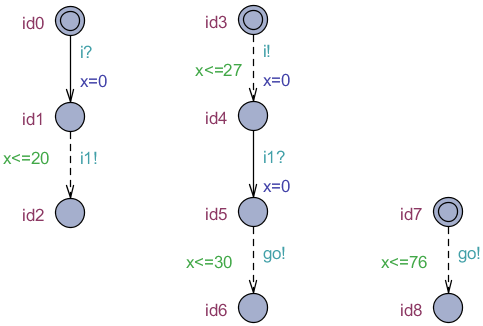
\includegraphics{figures/accum-delays.png}};
    \begin{scope}[x={(image.south east)},y={(image.north west)}]
        
        \node[font=\Large] at (0.70,0.2) {$\Scale[2]{{\leq}}$};
        \node[font=\Large] at (0.32,0.65) {$\Scale[2]{{\parallel}}$};
    \end{scope}
\end{tikzpicture}
\caption{Refinement, which requires accumulative delays} \label{fig:accDelay}
\end{figure}

\subsection{Implementation details}
After seeing the issue and the basic idea of how it can be solved with an example, one can take a look at the algorithm which computes the accumulation of delays. The function in Algorithm \ref{alg:accumDelay} demonstrates the main logic used to calculate the internal delays, given the source state and the target state.

The very first thing that is checked, in line 2, is if there was a reset, which is done by checking if the arrival min and max values are equal to zero. This check is important, because the accumulation of delays should happen only after reset, since time moves linearly and one can see the maximum delays within the guard zone. If the reset did not happen, we set the delay sum of the target state (DSum) to be equal to guard's maximum. In line 3, we check if guard maximum is infinity or if our current DSum is equal to infinity, then we set our target's DSum to be equal to infinity. The else statement in line 5 simply adds up the source DSum with guard's maximum and stores it in the target's DSum. This accumulation has to be performed on both sides of the refinement, since both sides can have internal moves.

\begin{algorithm}
\caption{Algorithm to compute accumulation of delays}
\label{alg:accumDelay}
\begin{algorithmic}[1]
\Function{accumulateDelays}{$sourceState, targetState$}
\If {$(aMin == 0 \And aMax == 0)$} 
    \If {$(source.DSum == INF \parallel gMax == INF)$}
        \State $target.DSum \gets INF;$
    \Else
        \State $target.DSum \gets source.DSum + gMax;$
    \EndIf
\Else 
    \State $target.DSum \gets gMax;$
\EndIf
        
\EndFunction
\end{algorithmic}
\end{algorithm}

At the end of the day, there were no significant issues while using accumulative delays. However after introducing a new concept, which is described in Section \ref{sec:globalZone}, there was no need for accumulative delays anymore. The reasoning behind this is that Global zone can handle it without any external help from such a function. 


\section{Timeline}
After facing such concepts as the absolute zone, Min/Max values and not being able to compare zones of the two sides of the refinement with the help of zone union subtraction, due to the possibly differing amount of clocks on each side, it was decided to introduce a \textit{flattening} abstraction.

The idea originated from previous discoveries: one is not able to compare zones of the left and right side of the refinement. The subtraction or intersection of the zones that is required to verify refinement rules did not appear possible to be performed, not only due to differing clock sizes of the refinement sides, but also because those clocks cannot be semantically compared (related to each other). 

As a result, it is necessary to compare the relationship of a set of an arbitrary amount of clocks with another such set. To achieve that, we introduce the concept of the \textit{timeline}, which in principle allows to flatten a multidimensional zone into a single dimension representing common results. Consider Figure \ref{fig:tl-1}, where a simplistic automaton has only one output edge, but three different clocks - \textit{x, y} and \textit{z}. Since location \textbf{id0} is the initial one and has no invariant assigned to it, the arrival and invariant zones of all three clocks evaluate to \textbf{0} and allow to indefinitely delay in that location respectively. The observation of the arrival zone of the location \textbf{id1} is of great interest: each of the clocks is constrained by the guards related to the rest of the clocks. This happens due to natural synchronous time progress that is identical for all of the clocks.

\begin{figure}
\centering
\begin{tikzpicture}[thick,scale=0.9, every node/.style={scale=0.9}]
    \node[anchor=south west,inner sep=0] (image) at (0,0)
    {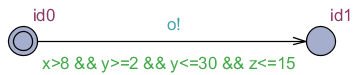
\includegraphics{figures/timeline-1.png}};
    \begin{scope}[x={(image.south east)},y={(image.north west)}]
        \node[font=\Large] at (0,1.4) {$\bm{x[0;0 ]}$};
        \node[font=\Large] at (0,1.1) {$\bm{y[0;0 ]}$};
        \node[font=\Large] at (0,0.8) {$\bm{z[0;0 ]}$};
        
        \node[font=\Large] at (0.02,0) {$\bm{x[0;\infty )}$};
        \node[font=\Large] at (0.02,-0.3) {$\bm{y[0;\infty )}$};
        \node[font=\Large] at (0.02,-0.6) {$\bm{z[0;\infty )}$};
        
        \node[font=\Large] at (0.3,-0.3) {$\bm{x(8;\infty )}$};
        \node[font=\Large] at (0.5,-0.3) {$\bm{y[2;30 ]}$};
        \node[font=\Large] at (0.7,-0.3) {$\bm{z[0;15 ]}$};
        
        \node[font=\Large] at (0.8,1.4) {$\bm{x(8;15 ]}$};
        \node[font=\Large] at (0.8,1.1) {$\bm{y(8;15 ]}$};
        \node[font=\Large] at (0.8,0.8) {$\bm{z(8;15 ]}$};
    \end{scope}
\end{tikzpicture}
\caption{Three clocks resulting is identical arrival zones after taking an edge} \label{fig:tl-aut}
\end{figure}

This observation evolved into the concept of flattening an arbitrary amount of clocks into a single "global" clock that represents all the possible clock valuations fot which an edge can be traversed. Figure \ref{fig:tl-1} shows an example of the timeline for the automaton in Figure \ref{fig:tl-aut}. Since the timeline can always be represented by one clock, we choose to draw it as an interval, where the values of the interval are derived from "tightest" guards. The semantics of the presented timeline is as follows: in order to traverse an edge from \textbf{id0} to \textbf{id1}, more than \textit{8} time units must pass ($x>8$ being the tightest lower bound constraint) and the edge remains traversable until \textit{15} ($z \leq 15$ being the tightest upper bound constraint).

\begin{figure}
\centering
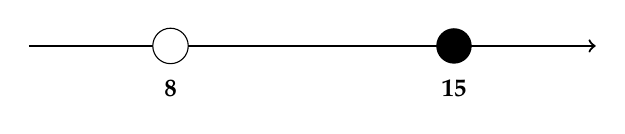
\begin{tikzpicture}[scale=0.9, every node/.style={scale=0.9}]
    \draw [thick ,->] (0,1) -- (8,1);
    \draw[fill=white] (2,1) circle (0.25);
    \node at (2,0.4) {$\bm{8}$};
    \fill (6,1) circle (0.25);
    \node at (6,0.4) {$\bm{15}$};
    \end{tikzpicture}

\caption{Timeline for the example in Figure \ref{fig:tl-aut}} \label{fig:tl-1}
\end{figure}

It is important to note that the concept of the timeline is also supposed to consider the fact that the refinement holds only when all the possible scenarios of state-space exploration satisfy its rules. The interval line(timeline) must reflect all the possible valuations that are common for all the clocks when the edge can be traversed, which includes all possible valuations for clocks derived from arrival zones.

\subsection{Implementation details}
To get a better intuition of what a timeline is and how it can be computed, consider the example in Figure \ref{fig:tl-plot}, where the arrival and guard zones are shown. As already mentioned, the arrival zone plays an important role in the computation of the resulting values of the timeline. 

\begin{figure}
\centering
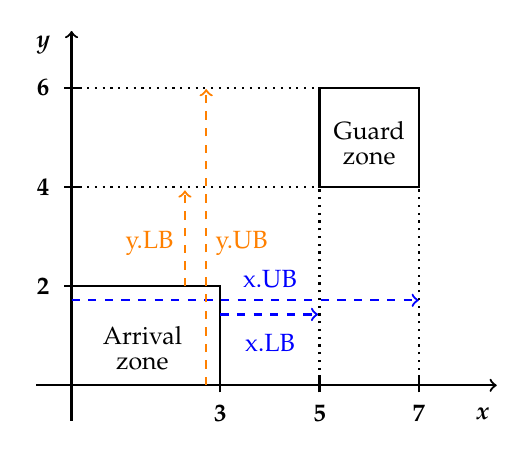
\begin{tikzpicture}[scale=0.9, every node/.style={scale=0.9}]
    % Axis
    \draw [thick ,->] (-0.5,0) -- (6,0);
    \draw [thick ,->] (0,-0.5) -- (0,5);
    \node at (5.8,-0.4) {$\bm{x}$};
    \node at (-0.4,4.8) {$\bm{y}$};
    
    % X coordinates
    \draw [thick] (2.1,-0.1) -- (2.1,0.1);
    \node at (2.1,-0.4) {$\bm{3}$};
    \draw [thick] (3.5,-0.1) -- (3.5,0.1);
    \node at (3.5,-0.4) {$\bm{5}$};
    \draw [thick] (4.9,-0.1) -- (4.9,0.1);
    \node at (4.9,-0.4) {$\bm{7}$};
    
    % Y coordinates
    \draw [thick] (-0.1,1.4) -- (0.1,1.4);
    \node at (-0.4,1.4) {$\bm{2}$};
    \draw [thick] (-0.1,2.8) -- (0.1,2.8);
    \node at (-0.4,2.8) {$\bm{4}$};
    \draw [thick] (-0.1,4.2) -- (0.1,4.2);
    \node at (-0.4,4.2) {$\bm{6}$};
    
    % Zones
    \draw [thick] (0,1.4) -- (2.1,1.4) -- (2.1, 0);
    \node at (1, 0.7) {Arrival};
    \node at (1, 0.3) {zone};
    \draw [thick] (3.5,2.8) -- (3.5,4.2) -- (4.9, 4.2) -- (4.9, 2.8) -- cycle;
    \node at (4.2, 3.6) {Guard};
    \node at (4.2, 3.2) {zone};
    
    % Dashed Arrows
    % Horizontal
    \draw [thick, blue, dashed, ->] (2.1,1) -- (3.48, 1);
    \draw [thick, blue, dashed, ->] (0,1.2) -- (4.9, 1.2);
    % Vertical
    \draw [thick, orange, dashed, ->] (1.9, 0) -- (1.9, 4.18);
    \draw [thick, orange, dashed, ->] (1.6,1.4) -- (1.6, 2.75);
    
    % Text on arrows
    \node[blue] at (2.8,0.6) {x.LB};
    \node[blue] at (2.8,1.5) {x.UB};
    
    \node[orange] at (1.1, 2) {y.LB};
    \node[orange] at (2.4, 2) {y.UB};
    
    % Dotted lines
    \draw [thick , dotted] (3.5,0) -- (3.5, 2.8);
    \draw [thick , dotted] (4.9,0) -- (4.9, 2.8);
    \draw [thick , dotted] (0,2.8) -- (3.5, 2.8);
    \draw [thick , dotted] (0,4.2) -- (3.5, 4.2);
    
\end{tikzpicture}
\caption{Computation of lower and upper bounds for further construction of a timeline.} \label{fig:tl-plot}
\end{figure}

Intuitively, the lower bound (LB) for a certain clock is the difference between the LB of the guard zone and the upper bound (UB) of the arrival zone for the respective clock. On the other hand, UB is the difference between the UB of the guard zone and the LB of the arrival zone for the respective clock.

Algorithm \ref{alg:timeline} demonstrates the computational process of the timeline. The idea is to compute the LBs and UBs for each of the clocks (Lines 4 and 5), and to pick the tightest bounds among all calculated LBs and UBs (Lines 10-13). The resulting two tightest bounds (final lower bound (FLB) and final upper bound (FUB) are the ones used to construct a timeline. Note that similarly to the previous algorithms, the difference between UB and LB is computed with the help of the addition function (\textsc{addRawRaw}), which is suitable due to the fact that the raw value of the LB is negative.

Also note that the resulting LB is expected to be a negative raw value, which is natural for all LBs. If the LB exceeds its allowed maximum value, it is set to the maximum value (Lines 6-7). This is a frequent example in cases where the arrival zone overlaps with the guard zone.

The UB also has its own minimum value, at most evaluating to \textbf{0} raw value. If the algorithm detects UB evaluating to negative raw values, it reports failure (Lines 8,9). This might happen in cases where the guard zone is "behind" the arrival zone in time, and therefore there are no clock valuations when an edge could be traversed.
\begin{algorithm}
\caption{Algorithm to compute timeline}
\label{alg:timeline}
\begin{algorithmic}[1]
\Function{getAbsoluteZone}{$arrZone, guardZone$}
\State $LB, UB, FLB = 1, FUB = Integer.MaxValue - 1;$
\ForAll{$clock$ in $zone$}
\State $LB \gets \textsc{addRawRaw}(arrZone.clockUB, guardZone.clockLB)$
\State $UB \gets \textsc{addRawRaw}(arrZone.clockLB, guardZone.clockUB)$
\If{($LB > 1$)}
\State $LB \gets 1$
\EndIf
\If{($UB < 1$)}
\State \textbf{return $null$}
\EndIf

\If{($LB < FLB$)}
\State $FLB \gets LB$
\EndIf
\If{($UB < FUB$)}
\State $FUB \gets UB$
\EndIf
\EndFor
\State
\State \textbf{return} new $Zone(1, FLB, FUB, 1)$
\EndFunction
\end{algorithmic}
\end{algorithm}

\subsection{Zone adjustment}
The timeline shows us absolute clock valuations during which an edge can be traversed and helps to verify if for all the solutions of one side of the refinement, the other side is able to "follow" by traversing an edge with the same action. However not only that, but the timeline can be used to adjust zones of both sides of the refinement.

Consider the automaton example in Figure \ref{fig:tl-autRight} which is the right side of the refinement, whereas the automaton of the left side of the refinement has been shown in Figure \ref{fig:tl-aut}. In order to construct a proper state pair of locations \textbf{id0} and \textbf{id3} for the refinement relation it is crucial to have proper zones to ensure the correctness of further state-space exploration, if any. 

The arrival zone at location \textbf{id3} in Figure \ref{fig:tl-autRight} which is depicted in red is an example of an incorrect zone in case of the refinement. Such zone would be correct if the automaton was explored outside the refinement relation or if it was on the left side of it. However, the timeline in Figure \ref{fig:tl-1} has shown that the output edge is traversed only in the interval of clock valuations from 8 (not included) until 15 (included). According to the refinement output rule, we are only interested in exploring such clock valuations on the right side as dictated by the left side. Therefore, the correct arrival zone would have to be $\bm{x(8;15]}$ (depicted in green).

\begin{figure}
\centering
\begin{tikzpicture}[thick,scale=0.9, every node/.style={scale=0.9}]
    \node[anchor=south west,inner sep=0] (image) at (0,0)
    {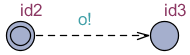
\includegraphics{figures/timeline-2.png}};
    \begin{scope}[x={(image.south east)},y={(image.north west)}]
        \node[font=\Large] at (-0.05,1) {$\bm{x[0;0 ]}$};
        \node[font=\Large] at (0.05,-0.2) {$\bm{x[0;\infty )}$};
        \node[font=\Large] at (0.5,0) {$\bm{x[0;\infty )}$};
        \node[font=\Large, green] at (0.7,1.25) {$\bm{x(8;15]}$};
        \node[font=\Large, red] at (0.7,0.85) {$\bm{x[0;\infty )}$};
        
    \end{scope}
\end{tikzpicture}
\caption{Automaton that is refined by the automaton from Figure \ref{fig:tl-aut}} \label{fig:tl-autRight}
\end{figure}

Such a  zone adjustment can be achieved by the following steps:
\begin{itemize}
    \item $LB_{AZ} = LB_{IZ} + LB_{timeline}$ \\
    To get the lower bound of the target arrival zone it is required to increase the source location invariant zone lower bound by the lower bound of the timeline.
    \item $UB_{AZ} = LB_{IZ} + UB_{timeline}$ \\
    Set the upper bound to be the same as the lower bound and then increase it by the upper bound of the timeline.
\end{itemize}

\subsection{Timeline issues}
In practice, the concept of timeline appeared to be capable of solving the same problems that absolute zones and min/max concepts did, but at a much more efficient and intuitive level. Unfortunately, it was discovered that the timeline has a number of flaws that prevent this concept from providing the expected results in some corner cases.

First of all, the information about the correct strictness may be lost after constructing a timeline. The example in Figure \ref{fig:tl-2} shows two cases where identical arrival zones and two different guard zones are used in each case to construct corresponding timelines. The resulting timelines appear to be identical, even though the strictness of the upper bound of the guards they were derived from differ. This is correct from the mathematical point of view, as the addition of two bounds, s.t. at least one of them is strict, will always result in a strict bound. However, in further computations that would result in incorrectly constructed arrival zones, as the information about exact strictness(one bound being non strict) is lost.


\begin{figure}
\centering
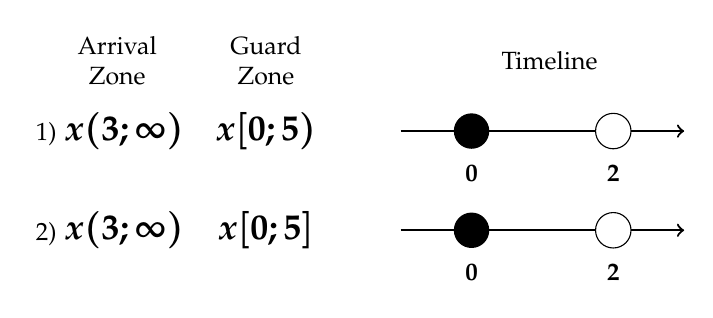
\begin{tikzpicture}[scale=0.9, every node/.style={scale=0.9}]

    \node[align=center] at (1,1) {Arrival \\ Zone};
    \node[align=center] at (3.1,1) {Guard \\ Zone};
    \node[align=center] at (7.1,1) {Timeline};
    \node at (0,-0.05) {1)};
    \node[font=\Large] at (1.1,0) {$\bm{x(3;\infty )}$};
    \node[font=\Large] at (3.1,0) {$\bm{x[0;5)}$};
    
    \node at (0,-1.45) {2)};
    \node[font=\Large] at (1.1,-1.4) {$\bm{x(3;\infty )}$};
    \node[font=\Large] at (3.1,-1.4) {$\bm{x[0;5]}$};
    
    
    \draw [thick ,->] (5,0) -- (9,0);
    \fill (6,0) circle (0.25);
    \draw[fill=white] (8,0) circle (0.25);
    \node at (6,-0.6) {$\bm{0}$};
    \node at (8,-0.6) {$\bm{2}$};
    
    \draw [thick ,->] (5,-1.4) -- (9,-1.4);
    \fill (6,-1.4) circle (0.25);
    \draw[fill=white] (8,-1.4) circle (0.25);
    \node at (6,-2) {$\bm{0}$};
    \node at (8,-2) {$\bm{2}$};
    \end{tikzpicture}

\caption{Two identical timelines for different strictness guards} \label{fig:tl-2}
\end{figure}

Secondly, we discovered that in some cases even if the timeline is correct, it does not anymore preserve the necessary information for the zone adjustment algorithm. Similarly to previous examples, Figure \ref{fig:tl-3} demonstrates four cases of arrival and guard zone combinations with varying strictness of the bounds. In fact, even though all the timelines are identical, they are absolutely correct according to their primary purpose. Each of them states that in all the possible scenarios of the state-space exploration joined together (which is driven by different arrival values), one might be able to traverse an edge immediately or to delay indefinitely and still be able to do so. However, such timeline is not suitable for proper zone adjustment as it has lost information about the necessary delay in some of the cases.

\begin{figure}
\centering
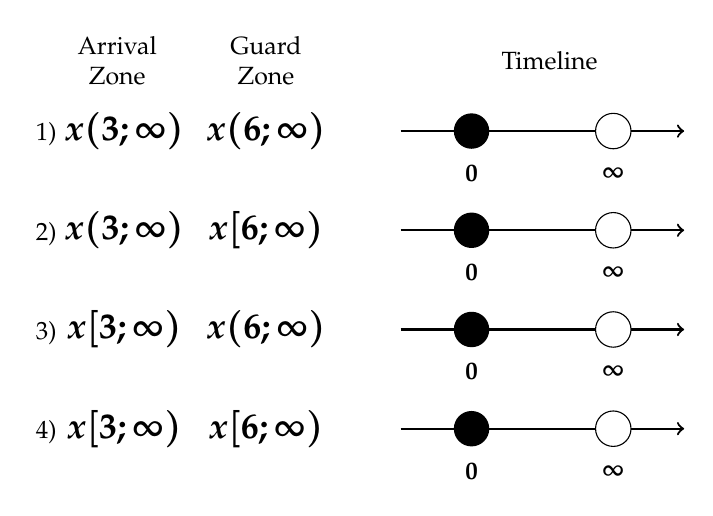
\begin{tikzpicture}[scale=0.9, every node/.style={scale=0.9}]

    \node[align=center] at (1,1) {Arrival \\ Zone};
    \node[align=center] at (3.1,1) {Guard \\ Zone};
    \node[align=center] at (7.1,1) {Timeline};
    \node at (0,-0.05) {1)};
    \node[font=\Large] at (1.1,0) {$\bm{x(3;\infty )}$};
    \node[font=\Large] at (3.1,0) {$\bm{x(6;\infty )}$};
    
    \node at (0,-1.45) {2)};
    \node[font=\Large] at (1.1,-1.4) {$\bm{x(3;\infty )}$};
    \node[font=\Large] at (3.1,-1.4) {$\bm{x[6;\infty )}$};
    
    \node at (0,-2.85) {3)};
    \node[font=\Large] at (1.1,-2.8) {$\bm{x[3;\infty )}$};
    \node[font=\Large] at (3.1,-2.8) {$\bm{x(6;\infty )}$};
    
    \node at (0,-4.25) {4)};
    \node[font=\Large] at (1.1,-4.2) {$\bm{x[3;\infty )}$};
    \node[font=\Large] at (3.1,-4.2) {$\bm{x[6;\infty )}$};
    
    
    \draw [thick ,->] (5,0) -- (9,0);
    \fill (6,0) circle (0.25);
    \draw[fill=white] (8,0) circle (0.25);
    \node at (6,-0.6) {$\bm{0}$};
    \node at (8,-0.6) {$\bm{\infty}$};
    
    \draw [thick ,->] (5,-1.4) -- (9,-1.4);
    \fill (6,-1.4) circle (0.25);
    \draw[fill=white] (8,-1.4) circle (0.25);
    \node at (6,-2) {$\bm{0}$};
    \node at (8,-2) {$\bm{\infty}$};
    
    \draw [thick ,->] (5,-2.8) -- (9,-2.8);
    \fill (6,-2.8) circle (0.25);
    \draw[fill=white] (8,-2.8) circle (0.25);
    \node at (6,-3.4) {$\bm{0}$};
    \node at (8,-3.4) {$\bm{\infty}$};
    
    \draw [thick ,->] (5,-4.2) -- (9,-4.2);
    \fill (6,-4.2) circle (0.25);
    \draw[fill=white] (8,-4.2) circle (0.25);
    \node at (6,-4.8) {$\bm{0}$};
    \node at (8,-4.8) {$\bm{\infty}$};
    \end{tikzpicture}

\caption{Four identical timelines for varying strictness of arrival and guard zones} \label{fig:tl-3}
\end{figure}

To fix these issues it would perhaps suffice to to enrich the timeline to be able to preserve more information that will be necessary in the phase of zone adjustment, however a new, more powerful concept was discovered.

\section{Global Zones}\label{sec:globalZone}
So far we have discussed a number of concepts such as arrival zone, Min/Max, accumulative delays and timeline, all of which shared similar problems - loss of information, impossibility of subtraction of opposite bound constraints and more. All of these previous concepts required a number of changes to perform correctly, however then they would become too unintuitive and cumbersome to implement.

This section presents the final concept that is used in the implementation of \jecdar - the one of the \textit{global zone}. As described in Section \ref{sec:refRules}, the refinement relation rules are applied on the pairs of the states that belong to the refinement relation. Each state in the state pair represents a number of corresponding locations and contains its own zone that keeps track of all clocks from relevant automata. It means that both left and right sides of the refinement (left and right states in the state pair) existed independently from each other. Having their own zones that could not be related or compared due to their potentially differing size, proper state-space exploration required some mechanisms for zone comparisons, all of which were described in previous sections.

Moreover, clocks of different sides of the refinement cannot be semantically compared. However, as was discovered later, such a mindset caught us locked in the tunnel vision trap.

\subsection{One common zone}
In fact, throughout the entire development of all the previous concepts, it appears that we were unconsciously trying to find various mechanism allowing us to compare every clock of the left side of the refinement to every clock on the right side. The "flattening" approach of the timeline was perhaps the closest concept to achieving that. Finally, the concept of a \textit{global} zone was born, which implies storing all clocks of the entire refinement in a single zone and thus having a single zone per refinement relation instead of two as before. 

The global zone helps to easily and efficiently solve a number of problems and allows us to freely use such DBM Library operations as \textsc{isSubsetEq}, \textsc{DbmMinusDbm} and \textsc{FedMinusFed} due to the global zone being of the same dimension (size) throughout the entire refinement. Moreover, storing all the clocks in one zone also implies constantly maintaining the relationship between any pair of clocks.

\subsection{Refinement rules verification}
With the global zone, the verification of refinement rules becomes a much more intuitive task. Consider the example in Figure \ref{fig:tl-refoutfail} where two automata are challenged to satisfy the refinement relation. The global zone, storing information about clocks of both sides of the refinement is used to verify refinement rules. For simplicity, axes \textbf{x} and \textbf{y} correspond to clocks \textbf{x} and \textbf{y} respectively. 

We know that the refinement output rule challenges an automaton on the right side of the relation to follow the left side with the same common output (in this example \textbf{o!}). To verify that, the global zone of the initial location is constrained by the corresponding guard ($x \leq 4)$ to obtain the zone of all the clock valuations when the output edge can be taken from \textbf{id0} to \textbf{id1} (zone on the left side). At this point, it is allowed to "cut" (constrain) the zone. Next, the resulting zone is then being constrained by the guard of the right side ($y \leq 2$). As can be seen on the right diagram of the zone (Figure \ref{fig:tl-refoutfail}), the application of the guard would not only constrain the clock of the right side \textbf{y}, but would also "cut" solutions from the clock of the left side \textbf{x}. This indicates that not for all the clock valuations an output can be taken on the left side so that the right side could follow. Therefore, refinement fails.

\begin{figure}
\centering
\begin{tikzpicture}[scale=0.9, every node/.style={scale=0.9}]
    %Automata
    \node at (1.6, 5.5) {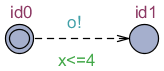
\includegraphics{figures/gz-aut1.png}};
    \node at (9.4, 5.5) {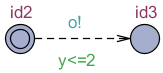
\includegraphics{figures/gz-aut2.png}};
    \node[font=\Large] at (5.5,5.5) {$\Scale[2]{{\leq}}$};

    % Axis
    \draw [thick ,->] (-0.5,0) -- (3.5,0);
    \draw [thick ,->] (0,-0.5) -- (0,3.5);
    \node at (3.5,-0.4) {$\bm{x}$};
    \node at (-0.4,3.5) {$\bm{y}$};
    
    % X coordinates
    \draw [thick] (1.4,-0.1) -- (1.4,0.1);
    \node at (1.4,-0.4) {$\bm{2}$};
    \draw [thick] (2.8,-0.1) -- (2.8,0.1);
    \node at (2.8,-0.4) {$\bm{4}$};
    
    % Y coordinates
    \draw [thick] (-0.1,1.4) -- (0.1,1.4);
    \node at (-0.4,1.4) {$\bm{2}$};
    \draw [thick] (-0.1,2.8) -- (0.1,2.8);
    \node at (-0.4,2.8) {$\bm{4}$};
    
    % Diagional Lines
    \draw [thick] (0,0) -- (2.8, 2.8);
    \draw [thick, dotted] (2.8, 2.8) -- (3.2, 3.2);
    \node[green] at (3.5,1.4) {$\bm{x \leq 4}$};
    
    % Dotted lines
    \draw [thick, green, dashed] (2.8,0) -- (2.8, 3.5);
    
    
    \node at (5.5, 1.4) {$\Longrightarrow$};
    
    %Second Plot
    % Axis
    \draw [thick ,->] (7.5,0) -- (11.5,0);
    \draw [thick ,->] (8,-0.5) -- (8,3.5);
    \draw [thick, red] (9.4,0) -- (10.8,0);
    \node at (11.5,-0.4) {$\bm{x}$};
    \node at (7.6,3.5) {$\bm{y}$};
    
    % X coordinates
    \draw [thick] (9.4,-0.1) -- (9.4,0.1);
    \node at (9.4,-0.4) {$\bm{2}$};
    \draw [thick] (10.8,-0.1) -- (10.8,0.1);
    \node at (10.8,-0.4) {$\bm{4}$};
    
    % Y coordinates
    \draw [thick] (7.9,1.4) -- (8.1,1.4);
    \node at (7.6,1.4) {$\bm{2}$};
    \draw [thick] (7.9,2.8) -- (8.1,2.8);
    \node at (7.6,2.8) {$\bm{4}$};
    
    % Diagonal Lines
    \draw [thick] (8,0) -- (9.4, 1.4);
    \draw [thick, red, dotted] (9.4, 1.4) -- (10.8, 2.8);
    \node[red] at (10.5,1.1) {$\bm{y \leq 2}$};
    
    % Dotted lines
    \draw [thick, red, dashed] (8,1.4) -- (11.5, 1.4);
    
\end{tikzpicture}
\caption{Refinement fails due to its output rule being not satisfied. Global zones illustrated after application of guards. Zone of the right side "cuts" solutions from the left side.} \label{fig:tl-refoutfail}
\end{figure}

Algorithmically, the easiest way to discover that a zone was "cut" is to make use of the subtraction operation \textsc{DbmMinusDbm} provided by the DBM Library. If the result of such a method call results in anything but an empty zone, it indicates that solutions were lost. Thus, the verification of the refinement output rule requires the subtraction of the right side global zone from the left side one, whereas the refinement input rule requires the opposite.

Moreover, the concept of the global zone removes any necessity to keep track of accumulative delays, which were described in Section \ref{sec:accumDelays}. This is due to the fact that zones contain not only lower and upper bounds of the clock, but also the relationship between any pair of clocks. In such cases as in Figure \ref{fig:accDelay}, if constructed properly the global zone would maintain the difference between clocks and the accumulative delays can then also be verified with the help of zone subtraction. A similar logic applies to the verification of the refinement delay rule, with a difference in subtraction being used on the global zones after the application of the corresponding invariants.

\subsection{Extrapolation}
During the verification of the refinement, the \textit{passed} list of states is used to guarantee termination. Whenever a new state is explored, it is checked against the existing \textit{passed} list with the following conditions: the locations of the compared states should be equal and the zone of the new state should be a subset of the state in the \textit{passed} list. If both of these conditions hold, the newly discovered state is considered as "already explored" and is discarded. This approach used to guarantee termination when each side of the refinement had its own zone.

However, the introduction of the global zones came along with another challenge. In some cases, the state-space exploration algorithms would no longer terminate due to the zone being infinitely incremented. Figure \ref{fig:gz-extrapolation} shows a simple example of this. Notice the invariant ($x \leq 1$) and the reset ($x=0$) that is present on the left side of the refinement, but not on the right. During state-space exploration we would expect the algorithm to terminate as in principle no new zones or locations are discovered even after the first traversal of \textbf{o!} edge on any side. However this is not the case for the global zones.

\begin{figure}
\centering
\begin{tikzpicture}[scale=0.9, every node/.style={scale=0.9}]
    %Automata
    \node at (0, 0) {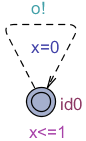
\includegraphics{figures/gz-extr-a1.png}};
    \node at (5, 0.25) {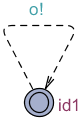
\includegraphics{figures/gz-extr-a2.png}};
    \node[font=\Large] at (2.5,0) {$\Scale[2]{{\leq}}$};
    
\end{tikzpicture}
\caption{Refinement example that requires extrapolation techniques to terminate.} \label{fig:gz-extrapolation}
\end{figure}

Since global zones also preserve information about relationship between clocks during the state-space exploration, the zone would keep progressively moving upwards on the \textbf{y} axis. Thus, the termination of the algorithm would not be possible due to an infinite number of symbolic states. 

To cope with this problem in \jecdar, a zone-based abstraction technique, also known as \textit{extrapolation}, (\textcite{ExtrapolationLU}) is used. Apart from \uppaal, extrapolation is also used in such tools as \textsc{Kronos} and \textsc{RtSpin} where it is referred to as \textit{maximization} (\textcite{maximization}). While preserving reachability properties, extrapolation greatly reduces the state-space that needs to be explored.

Extrapolation is based on the idea that the outcome of the feature verification for automata is only affected by the changes to a clock if its value is below some certain constant. As soon as the clock has surpassed the constant its values become irrelevant, i. e. all further resulting states are identical except for clock valuations exceeding the maximum constant. 

The selection of the maximal constants for clocks is an important matter as it influences the coarseness of the abstraction - the smaller the constant, the smaller state-space that has to be explored and less time and memory has to be used for the  verification of properties. 
The choice of the constant $k$ involves static analysis of the automaton with the aim of finding the maximal constant appearing in either guards or invariants within the structure of the automaton. Currently \jecdar finds one such constant for each of the clocks, which is a much coarser abstraction that using a single constant. In the example of Figure \ref{fig:gz-extrapolation} the maximal such constant for clock \textbf{x} is $k = 1$. As soon as the upper bound of that clock in the zone is greater than $k$ it is considered insignificant and can be replaced by a higher value being either the next highest upper bound of any another clock in the zone or an infinity if none. 

The idea of extrapolation has also been taken further in a number of studies to construct coarser yet exact abstractions. For example in \textcite{StaticGuardAnalysis} in addition to a constant depending on a particular clock it also depends on a particular location of the automaton. However, the current implementation of \jecdar makes use of the extrapolation based on the maximal constants for clocks, which is a potential subject for improvement in the future work.
\chapter{Implementation}\label{ch:impl}
This Chapter presents the set of features that were implemented, while providing an explanation regarding their necessity and specific details about how they were created.


\section{Nested features}
The task that had the highest priority was to make it possible to handle nested features, a functionality that had not been supported earlier, as mentioned in \textcite{Jecdar:2019}. The first version of \jecdar was able to handle composition and conjunction of simple automata (e.g., Administration || Machine || Researcher or HalfAdm1 \&\& HalfAdm2), but nesting such features was out of its scope.

We understood that handling such an issue would require changes in our data structures. A state used to be represented as a vector of locations (where each location would correspond to an automaton) and a zone. When trying to retrieve the next possible transitions that can be taken from a certain state, we would have to gather all the transitions that can be taken by each subcomponent. With a flat structure of the current location, this is hard to achieve, as we no longer know which part of the location corresponds to which transition system.

\begin{figure}
  \centering
  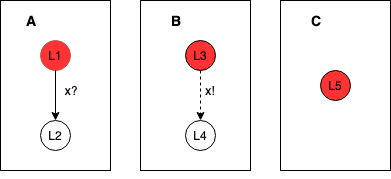
\includegraphics[scale=0.7]{figures/nestedLoc.png}
  \caption{(A || B) || C}
  \label{fig:nestedLoc}
\end{figure}

Figure \ref{fig:nestedLoc} illustrates this problem. It shows a composition between another composition (A || B) and a simple automaton, C. Note that, for simplicity, only the relevant parts of the automata are displayed. The red locations represent the current location. Being in the state consisting of locations L1, L3 and L5, we would like to know what transitions can be taken with the action x. If our location was simply represented as a vector of locations, we would not know which part of it we need in order to fetch the next transitions from (A||B) and from C.

\begin{figure}
  \centering
  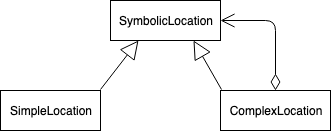
\includegraphics[scale=0.7]{figures/nestedness.png}
  \caption{Structure of the SymbolicLocation class}
  \label{fig:nestedness}
\end{figure}

We solved this issue by refactoring our location vector into what we call a "symbolic location". This new data type is represented by an abstract class, with two classes inheriting from it, as shown in Figure \ref{fig:nestedness}. A SymbolicLocation can be either a SimpleLocation or a ComplexLocation. A SimpleLocation is simply a wrapper for a regular Location, while a ComplexLocation can have many SymbolicLocations.

\begin{figure}
  \centering
  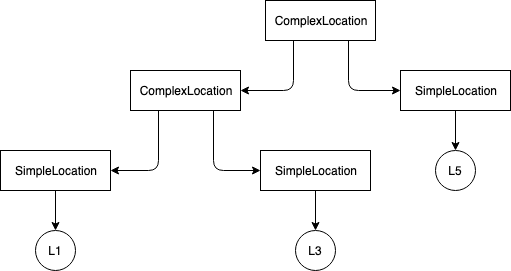
\includegraphics[scale=0.7]{figures/symbolicLoc.png}
  \caption{Tree representation of a location}
  \label{fig:symbolicLoc}
\end{figure}

This approach allows us to store locations as tree structures than can be built in a recursive fashion. Figure \ref{fig:symbolicLoc} shows how the location from (A || B) || C is represented in terms of the new data structure.

\begin{figure}
  \centering
  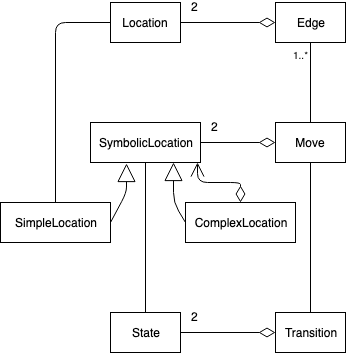
\includegraphics[scale=0.7]{figures/umlTransitions.png}
  \caption{Class diagram}
  \label{fig:umlTransitions}
\end{figure}

Moreover, if we previously used to retrieve outgoing edges from a location, after introducing symbolic locations we discovered the need to create a corresponding abstraction for outgoing edges from a symbolic location. We gave this new concept the name of "Move", and its purpose is to connect two symbolic locations through a vector of edges. This way, we can get the moves that can be taken from each symbolic location of a certain state and then aggregate them in order to build a transition. Figure \ref{fig:umlTransitions} presents the correlation between states, symbolic locations and locations and the one between transitions, moves and edges.


\section{Addition of strictness} \label{sec:strictnessFix}

As explained in \textcite{Jecdar:2019}, since transition systems can be infinite due to an infinite amount of states given by time being continuous, we must use a symbolic representation of states in order to achieve finiteness. A common approach is to make use of zones, which contain intervals for each clock, and this is also the approach that we chose. We represent zones through DBMs (difference bound matrices), which allow us to specify the upper bound on the difference between each two clocks. 

\begin{figure}
  \centering
  \includegraphics[scale=0.7]{figures/strictness.png}
  \caption{Conversion from actual DBM to internal representation}
  \label{fig:strictness}
\end{figure}

The DBM library allows us to construct such constraints and to specify their strictness (< or $\leq$). The value and its strictness are encoded in each constraint. We noticed that we were building DBMs incorrectly, as by default all our constraints were non strict and we used to modify the values in order to match the strictness (e.g., $x < 7$ would be turned into $x \leq 6$, which means that the values from the interval (6, 7) would be omitted).

In Figure \ref{fig:strictness} we show an example of an actual DBM and how the previous version of \jecdar used to adjust the values according to the strictness and then convert it into the library's internal representation. We also illustrate the correct representation that we now achieve by eliminating the adjustment and encoding each constraint according to its strictness.

\section{XML Parser}

The first version of \jecdar had a JSON parser for the models created with \ecdar 2.x. In order to automate our tests as much as possible, it was important to avoid creating test cases manually. The most suitable approach that we found was to create models in \ecdar 2.x, which can later be parsed into our internal data structures that the tests can be run on. We would run different queries on these models and use the results to infer the expected output of each test. Our reason for choosing \ecdar 2.x was the fact that it was our intention to integrate \jecdar with the new GUI at a later point, so it made sense to use it for creating models and verifying properties of them.

After experiencing questionable results when running certain queries, we decided to check whether \ecdar 0.10 would provide us with different outputs. As expected, \ecdar 0.10 gave the same results, and that makes sense since both versions are using the same engine behind the scenes. However, \ecdar 0.10 would also display handy error messages. (e.g., the reason why a refinement holds or does not hold).

Henceforth, we made the decision to continue creating and testing models in \ecdar 0.10 and for that purpose we found it useful to create an XML parser as well. 

This parser is implemented in a similar way to the JSON one. It uses a library in order to simplify the task and to reduce the chances of making mistakes. The parsing is performed by taking a specific XML file and operating on the nodes corresponding to the automata. The result is a list of automata that together make up a model.

Moreover, since we now support models in XML format as well, we introduced one additional thing. As mentioned in \textcite{Jecdar:2019}, we have several commands that can be used for communicating with \jecdar from the terminal. The "-rq folderPath query query..." command, which runs one or more queries, given the path of the model, has been modified with the addition of an extra flag to indicate whether the model is in JSON or in XML format. The reason for doing is so that the controller can decide which parser it should use. In order to run such a command, "-rq" must be typed, followed by either "-json" or "-xml", followed by the actual queries.

\section{Determinism check} \label{sec:implDeterm}
According to \textcite{David:2010}, the specification theory was defined to be applied on deterministic TIOTS, where the following applies: for all $a \in \Sigma \cup \mathbb{R}_{\geq 0}$ whenever $s\xrightarrow{a}^S s'$ and $s\xrightarrow{a}^S s''$ we have $s' = s''$. Without this property, one would not be able to tell which edge has to be taken for an action. Therefore, a determinism must be ensured for each of the automaton and is considered an implicit prerequisite for any further application of features on that automaton.

To check for the determinism property of an automaton, one must ensure there does not exist a non-deterministic choice on an action (edge) at any location of the automaton. The Algorithm \ref{alg:isDeterministic} outlines the general implementation design for the determinism check.

\begin{algorithm}
\caption{Algorithm to verify determinism of automaton}
\label{alg:isDeterministic}
\begin{algorithmic}[1]
\Function{isDeterministic}{}
\State $Passed \gets \{\}$ 
\State $Waiting \gets \textsc{getInitialState()}$
\While{$(Waiting.hasNext)$}
    \State $state \gets Waiting.\textsc{pop}()$
    \State $passed.\textsc{add}(state)$
    \ForAll{$action$ in $actions$}
        \State $trans \gets \textsc{GetNextTransitions}(state, action)$
        \If{($\textsc{CheckMovesOverlap}(trans)$)}
            \State \textbf{return $false$}
        \Else
        \State $targets \gets (tran::\textsc{getTarget}) \notin passed $
        \State add $targets$ to $Waiting$
        \EndIf
    \EndFor
\EndWhile
\State
\State \textbf{return $true$} 
\EndFunction
\end{algorithmic}
\end{algorithm}

The idea is to check every reachable location of the automaton, but do that only once. For that, \textit{passed} and \textit{waiting} lists are used. Then for each location in the \textit{waiting} list the following applies: a) the location is moved to the \textit{passed} list, b) for each action, present in the signature of the automaton, the possible transitions are acquired, c) actions are checked for determinism (Line 9). As soon as at least a single instance of non-determinism is encountered the algorithm reports determinism to have failed (Line 10). 

Algorithm \ref{alg:moves-overlap} shows the logic behind the \textsc{CheckMovesOverlap} method. The idea behind the verification of an arbitrary amount of transitions for their "overlapping" lies in ensuring there is no intersection between all possible combinations of two transitions.

\begin{algorithm}
\caption{Algorithm to check if transitions overlap}
\label{alg:moves-overlap}
\begin{algorithmic}[1]
\Function{CheckMovesOverlap}{$trans$}
\If{($trans.size < 2$)}
    \State \textbf{return $false$};
\EndIf
    \For{($i\gets 0; i < trans.size; i++$)}
        \For{($j\gets i+1; i < trans.size; i++$)}
        \If{(trans[i].targetLoc = trans[j].targetLoc)}
        \If{(trans[i].\textsc{hasEqualUpdates}(trans[j])}
        \State \textbf{continue}
        \EndIf
        \EndIf
        \State $zone1 \gets$ trans[i].targetLoc.invZone
        \State $zone2 \gets$ trans[j].targetLoc.invZone
            \If{(\textsc{intersect}($zone1, zone2$))}
            \State \textbf{return $true$}
            \EndIf
        \EndFor
    \EndFor
\State
\State \textbf{return $false$}	
\EndFunction
\end{algorithmic}
\end{algorithm}

In principle, a single existing transition cannot create non-determinism (Lines 2-3). For a larger amount of transitions, the algorithm takes a look at every possible pair of transitions without considering the same pair more than once. Note that if a considered pair of transitions leads to the same target location and the updates (resets) of those two transitions are identical it should be considered a deterministic pair and not checked for intersection (Lines 6-8). In other words, even if two transitions lead to the same location, but their updates (resets) differ, they may create a non-deterministic choice in terms of zones for clocks if these transitions overlap.

Next, for each pair the intersection of zones is checked and if one exists then the algorithm reports non-determinism. This algorithm eliminates the problem present in \ecdar 0.10 which was described in Section \ref{sec:determBug}.

\section{Consistency check}

The determinism check is a prerequisite for the next feature implemented - consistency check. In fact, all automata must first pass the determinism check before being eligible for any further computations.

The Algorithm \ref{alg:check-consistency} is suitable for checking two types of consistency: least fixpoint consistency and full consistency, both of which were mentioned in Section \ref{sec:minConsistency}. The type of consistency to be checked is determined by the boolean variable \textit{canPrune} that is passed as an argument to the \textsc{CheckConsistency} method together with the \textit{state} from which the consistency check should begin, normally being the initial state.

This algorithm has a recursive nature and avoids loops in the structure of the automaton by maintaining the list of $passed$ states. Any state that is checked for consistency will either be added to the \textit{passed} list or return \textit{true} if the state has been already explored (Lines 2-4). 

\begin{algorithm}
\caption{Algorithm to check consistency}
\label{alg:check-consistency}
\begin{algorithmic}[1]
\Function{CheckConsistency}{$state, canPrune$}
\If{($state \in passed$)} 
\State \textbf{return} true;
\EndIf
\State add $state$ to $passed$
    \ForAll{$action$ in $inputs$}
    \State $trans \gets \textsc{GetNextTransitions}(state, action)$
        \ForAll{$tran$ in $trans$}
            \If{($\neg$\textsc{CheckConsistency}($tran.Target, canPrune$))}
            \State \textbf{return $false$};
            \EndIf
        \EndFor
    \EndFor
    \State
    \If{($canPrune$ and $state.\textsc{CanDelayIndefinitely}$)}
    \State \textbf{return $true$}
    \EndIf
    \State
    \ForAll{$action$ in $outputs$}
        \State $trans \gets \textsc{GetNextTransitions}(state, action)$
        \ForAll{$tran$ in $trans$}
            \State $isConsistent \gets \textsc{CheckConsistency}(state, canPrune)$
            \If{($consistent$ and $canPrune$)}
            \State \textbf{return $true$}
            \EndIf
            \If{($\neg consistent$ and $\neg canPrune$)}
            \State \textbf{return $false$}
            \EndIf
        \EndFor
    \EndFor
    \State
    \If{($\neg canPrune$)}
        \If{($outputExisted$)}
        \State \textbf{return $true$}
        \Else
        \State \textbf{return} $state.\textsc{CanDelayIndefinitely}$
        \EndIf
    \EndIf
    
\State
\State \textbf{return $false$}	
\EndFunction
\end{algorithmic}
\end{algorithm}

Lines 5 to 9 handle all the outgoing input edges from the current state. As mentioned in Section \ref{sec:minConsistency}, inputs cannot be assumed to never be received as they depend on the unpredictable environment. Therefore regardless of being allowed to prune inconsistent parts of the automaton or not, the targets of those input edges must always be checked for consistency. If the target state of at least one input edge appears to be inconsistent, the entire check of consistency returns \textit{false} (Lines 8-9).

Interestingly, with the least fixpoint consistency it suffices to find the earliest state that satisfies the property of independent progress and simply prune the rest. In such cases, when the consistency check is allowed to prune, the two lines 11 and 12 are executed. The algorithm returns \textit{true} if independent progress property is satisfied by the state being able to delay indefinitely.

If the state was not able to delay indefinitely or the pruning was not allowed, the algorithm proceeds to checking all the outgoing output edges. Each outgoing edge is checked for consistency by performing a recursive call and the boolean result is stored in the \textit{isConsistent} variable (Line 17). In the case of being allowed to prune states, having found at least a single consistent state suffices for the entire consistency check to return $true$ (Lines 18-19). On the other hand, not being able to prune states and having found at least one inconsistent state reached by an output edge means not satisfying the consistency check (Lines 20-21).

After having checked both input and output edges of the state there is some logic left for cases of computing full consistency. If an output edge existed at that state and we have not found any inconsistent states reached by any edges, the algorithm is safe to report the automaton being consistent(Lines 24-25). However, if no outputs existed, the only way to ensure the independent progress property becomes the possibility of the state to delay indefinitely (Lines 26-27). 

Finally, if by the very end of the algorithm none of the return statements were triggered, it means that no states managed to satisfy the property of independent progress and, therefore, the algorithm terminates.

\section{Implementation feature}
The feature of verifying whether an automaton is an \textit{Implementation} is the next step from consistency check. In general, the implementation feature is "stricter" than the consistency check by one extra property: in addition to determinism and consistency checks the automaton has to ensure the property of output urgency.

\begin{algorithm}
\caption{Algorithm to verify the implementation property}
\label{alg:isImplementation}
\begin{algorithmic}[1]
\Function{isImplementation}{}
\State $Passed \gets \{\}$ 
\State $Waiting \gets \textsc{getInitialState()}$
\While{$(Waiting.hasNext)$}
    \State $state \gets Waiting.\textsc{pop}()$
    \State $passed.\textsc{add}(state)$
    \ForAll{$action$ in $actions$}
        \State $trans \gets \textsc{GetNextTransitions}(state, action)$
        \If{($\neg trans.\textsc{isEmpty}()$ and $action \in outputs$)}
            \If{($\neg \textsc{OutputsAreUrgent}(trans)$)}
            \State \textbf{return $false$}
            \EndIf
        \EndIf
        \State $targets \gets (tran::\textsc{getTarget}) \notin passed $
        \State add $targets$ to $Waiting$
    \EndFor
\EndWhile
\State
\State \textbf{return $true$} 
\EndFunction
\end{algorithmic}
\end{algorithm}

Since the algorithms for the determinism and consistency properties have already been demonstrated in previous sections, it is the output urgency property that is of interest. The verification of this property is shown in Algorithm \ref{alg:isImplementation}. The prerequisite for this algorithm is to be applied on the automaton that is already deterministic and fully consistent.

Similarly to the determinism check, this algorithm must consider every state only once which is done with the help of the \textit{waiting} and \textit{passed} lists. While iterating through all the states, only the edges that are of an output action matter. For each of such edges we then check if the output urgency property is preserved. This is done with the help of the \textsc{OutputsAreUrgent} method that ensures that there is no possibility to delay, but only to output immediately. 


\section{Federations and operations}

In the DBM library, there exists a data type that is used for representing unions of zones, and that is the Federation. Internally, this is simply an abstraction over a list of DBMs which is stored as two-dimensional arrays, where each array contains values of a certain DBM and all of the arrays (DBMs) must be of the same size.

Federations provide a wide selection of operations that can be applied on them, but the most interesting ones for our purposes are the ability to subtract a federation from a DBM, a DBM from a federation and a federation from a federation.

In order to call the DBM library, which is written in C/C++ from our Java code, we followed the same approach as before. We made use of the Java Native Interface, which made it very easy given that it was already set up, so we were able to add new methods quickly. The only aspect that made it challenging was to implement a mechanism for conversion between C++ objects and Java objects (and vice versa). Whenever we pass a federation to the library, we must convert it from Java to C++ and whenever we want to return a federation generated by the library, we must convert it from C++ to Java. 

Moreover, we found it relevant to create our own data type for a Federation, in order to achieve a higher level of abstraction. Figure \ref{fig:federation} illustrates, side by side, the internal representation of the Federation type in Java and in C++.

\begin{figure}
  \centering
  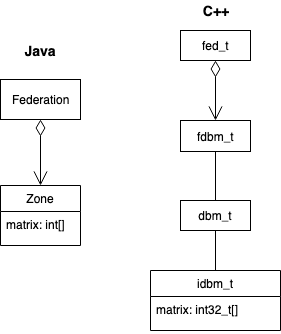
\includegraphics[scale=0.7]{figures/federation.png}
  \caption{Java vs C++ representation of a federation}
  \label{fig:federation}
\end{figure}

\section{Using federations to detect missing intervals}

When performing a refinement check, we must check for the input, output and delay rule. Since refinement is a binary relation, this must be done for each of the pairs belonging to the relation. 

Let (s, t) be the pair consisting of the initial states of the transition systems derived from S and T, shown in Figure \ref{fig:missingIntervals}. Since we have an output transition from s defined for valuations of x in the interval [20, 50], the same should hold for t in order for refinement to hold. However, in the case of t, the output transition is defined only for $[20, 30] \cup [40, 50]$, which means that we need a mechanism for determining that the (30, 40) interval is missing. 

One of our first ideas was to check the minimum and the maximum value for which the transition is enabled. This approach would fail, as the missing interval would not be caught.

An approach that would catch missing intervals is to use subtraction of federations. This involves building a federation with zones corresponding to all edges of a given action for one of the sides and then doing the same thing for the other side. Depending on whether it is an input or an output action, we subtract one federation from the other and if the resulting federation is not empty, then we can conclude that the rule is violated.

\begin{figure}
  \centering
  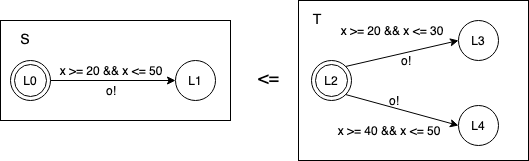
\includegraphics[scale=0.7]{figures/missingIntervals.png}
  \caption{S does not refine T}
  \label{fig:missingIntervals}
\end{figure}

\section{Input-enabledness}

After concluding that each transition system should be a specification by default, we realized the need to treat each state of a transition system as if it was input-enabled.

An automaton like the one in Figure \ref{fig:beforeInputEnabledness} derives a transition system that is not a specification, as not all states are input-enabled. State (L0, \{$x \in [0, \infty)$, $y \in [0, \infty)$\}) can only accept input i1 for values of x and y lower than 10 (included) and input i2 can be taken only for values of x and y higher than 3 (included). Moreover, the states corresponding to locations L1 and L2 do not accept any inputs.

\begin{figure}
  \centering
  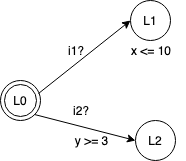
\includegraphics[scale=0.7]{figures/inputEnablednessBefore.png}
  \caption{Automaton resulting in transition system that is not a specification}
  \label{fig:beforeInputEnabledness}
\end{figure}

If we were to modify the previous automaton so that it would derive a specification, it would look like the one in Figure \ref{fig:afterInputEnabledness}. This automaton has all the missing self-loops added to each location, in order to ensure input-enabledness.

\begin{figure}
  \centering
  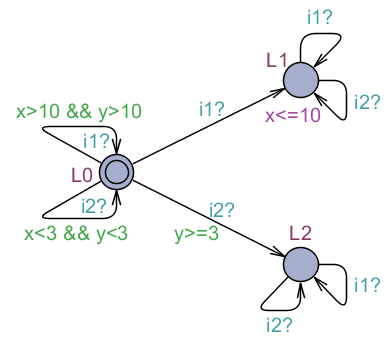
\includegraphics[scale=0.7]{figures/inputEnablednessAfter.png}
  \caption{Automaton resulting in transition system that is a specification}
  \label{fig:afterInputEnabledness}
\end{figure}

We discovered two ways of tackling the issue of input-enabledness: either to add the missing input transitions for each state whenever we try to fetch the next transitions from that state, or to perform the operation of adding the missing input edges to each automaton the moment that it is constructed.

While the former is somewhat easier to implement, the disadvantage is that the action would be repeated each time the next transitions for a state are requested. The latter, on the other hand, is an operation that only needs to be done once and this was a strong reason to choose it. Moreover, to simplify this task, we also opted for adding the invariant of the target location to each edge, as this makes it easier to understand the zone for which a certain input can be received and then derive the missing zones. In case there are resets on the edge, this step is skipped, as the invariant will always be satisfied.

\begin{algorithm}[H]
\caption{Apply input-enabledness function}
\label{alg:apply-input-enabledness}
\begin{algorithmic}[1]
\Function{ApplyInputEnabledness}{}
\ForAll{$loc$ in $locations$}
    \State $zone \gets initializeZone()$
    \State
    \ForAll{$invariant$ in $loc.Invariants$}
        \State $zone.\textsc{buildConstraintsForGuard}(invariant)$
    \EndFor
    \State $fullFederation \gets \{zone\}$
    \State
    \ForAll{$input$ in $inputs$}
        \State $inputEdges \gets \textsc{getEdgesFromLocation}(loc, input)$
        \State $zones \gets \{\}$
        \ForAll{$edge$ in $inputEdges$}
            \State $guardZone \gets zone$
            \ForAll{$guard$ in $edge.Guards$}
                \State $guardZone.\textsc{buildConstraintsForGuard}(guard)$
            \EndFor
            \State add $guardZone$ to $zones$
        \EndFor
        \State
        \State $federation \gets zones$
        \State $resultFederation \gets fullFederation - federation$
        \State
        \ForAll{$zone$ in $edgeZones$}
            \State $newEdge \gets$ (loc, loc, input, \textsc{buildGuardsFromZone}(edgeZone))
            \State add $newEdge$ to $edges$
        \EndFor
    \EndFor
\EndFor
\EndFunction
\end{algorithmic}
\end{algorithm}

Our implementation of the \textsc{ApplyInputEnabledness()} function is shown in Algorithm \ref{alg:apply-input-enabledness}. It starts out by iterating over all locations of an automaton, building a zone with the help of the invariants and using it to construct the federation belonging to that state. Then it looks at all the input edges corresponding to a single action and builds a federation consisting of a zone for each edge. In order to get the missing zones, this federation is subtracted from the full federation built in the beginning. The result of the subtraction is then used to build an edge for each zone and add it to the automaton's edges.

\section{Duplicate automata in refinement query} \label{sec:dupProc}

When running a refinement query, if the same automaton is present more than once on either side of the refinement, then problems can arise. Such a scenario can occur in a self refinement query, but also in more complex queries containing compositions or conjunctions. The main issue that we discovered is in the manipulation of zones, as applying constraints and updates on a clock will do that on the first occurrence of said clock, which is not necessarily the correct occurrence, as the same automaton can appear multiple times.

One solution to this problem would be to make a deep copy of each automaton whenever it is seen, given that it is not its first occurrence. This way we can ensure that the set of clocks of an automaton and the set of clocks of its copy are not the same, so we have a reference to the clock of the right automaton.

Another solution is to display an error message, in the style of \ecdar 0.10, which reports a "Duplicate process instance" error and points to the automaton that appears more than once in the query.

We found both approaches reasonable and estimated that they would require roughly the same time to implement. In order to maintain a consistency between \jecdar and \ecdar wherever it is sensible, we opted for reporting an error message in queries containing duplicate instances of an automaton.

\section{Error logging}

While \ecdar 2.x simply returns "yes", "no" or "maybe" as the result of a query, \ecdar 0.10 provides the user with significantly more feedback, namely it decides whether a query passes or fails, and in case of the latter it displays an error message pointing to the reasons why the chosen query did not succeed. Such messages include stating that there is a duplicate process instance, as presented in Section \ref{sec:dupProc}, or that an automaton is inconsistent.

We believe that offering the user the chance to see why a certain query has failed brings value and can contribute to the construction of correct models. For this reason, error messages were added to \jecdar.

This modification requires the different queries to check for all preconditions instead of terminating when the first issue is encountered. If any of the preconditions fails, then the refinement check is not run and the query fails, as expected. Having to check all preconditions can decrease performance in situations where the first issue is discovered early in the process, however it provides feedback and we think this trade-off is justified in the long run, especially as the size of models increases and they become harder to debug.

Figure \ref{fig:errLog} shows an example of the error messages that \jecdar returns when a query fails.

\begin{figure}
    \centering
    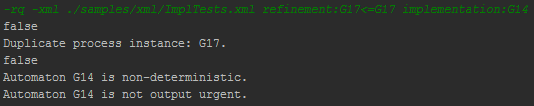
\includegraphics[scale = 0.7]{figures/ErrorMessages.png}
    \caption{Error logging example for multiple queries.}
    \label{fig:errLog}
\end{figure}

\section{Jecdar commands}
As mentioned in \textcite{Jecdar:2019}, we have several commands that can be used for communicating with \jecdar from the terminal. The list of commands can be seen in Table \ref{tbl:commands}. The "-rq folderPath query query..." command, which runs one or more queries, given the path of the model, has been modified with the addition of an extra flag to indicate whether the model is in JSON or in XML format. The reason for doing is so that the controller can decide which parser it should use. In order to run such a command, "-rq" must be typed, followed by either "-json" or "-xml", followed by the actual queries.

An important notice one shall take, that \jecdar is now capable of recognising such keywords as determinism, consistency and implementation. One may simply invoke the "-rq" command and in the query specify that they want to get determinism check results. An example of such query could be "determinism:Machine", running this query will show if the automaton is deterministic.

In \ecdar 0.10 and \ecdar 2.x the determisnm check as a stand alone check does not exists, however it is included in the consistency as well implemen
%In addition to the previously mentioned commands, there were introduced two new commands in order to be able to return the Refinement relation as well as Refinement trace if the check return false. Table \ref{tbl:newCommands} provides with the list of new commands added to \jecdar. It is important that one would keep in mind to provide with the corresponding flag, which indicates whether it is JSON or XML format. The "-rqrr" command returns the refinement relation in a tree format as well as the result if it fails or not.

\begin{center}
\begin{table}
    \begin{tabular}{ | l | p{6cm} |}
    \hline
    Commands & Description of commands\\ \hline \hline
\textbf{-help} &This command provides a list of all \jecdar commands as well as their usage\\ 
\hline
\textbf{-version} &Returns the current version of the engine.\\ 
\hline
\textbf{-vq query} &Given a query this command will verify if the query is syntactically correct.\\
\hline

\textbf{-rq -json/-xml folderPath query query...} &Given a folder location with indicator for the format of the files and one or more queries this command will firstly check if the queries are syntactically correct and then will run them.\\ 

\hline
    \end{tabular}
    \caption{\jecdar commands \textcite{Jecdar:2019}}
     \label{tbl:commands}
     \end{table}
\end{center}




\iffalse
\begin{center}
\begin{table}
    \begin{tabular}{ | l | p{5.7cm} |}
    \hline
    Commands & Description of commands\\ \hline \hline
\textbf{-rqrr -json/-xml folderPath query query...} &This command works very alike to -rq, except it returns the refinement relation. Given a folder location with indicator for the format and one or more queries this command will execute the check and return the refinement relation.\\ 
\hline
\textbf{-rqrt -json/-xml folderPath query query...} &This command works almost the same as -rqrr, however instead of returning refinement relation, it will return trace to where the refinement check failed.\\ 
\hline
    \end{tabular}
    \caption{New \jecdar commands}
     \label{tbl:newCommands}
     \end{table}
\end{center}
\fi


\chapter{Testing}\label{ch:testing}
In this chapter we describe the testing approach as well as some specific examples of testing scenarios that help us to validate correctness and quality. The testing experience from the previous semester of \jecdar development, which included over 130 tests with an overall code coverage being at least 95 percent, has proven to be insufficient to detect some of the refinement problems. Therefore, we have introduced a number of case specific tests with the aim of testing every potential corner case of both previously existing and newly implemented features.

These test cases include all of the examples described in Chapters \ref{ch:inconst} and \ref{ch:concepts}, as well as a number of their variations with potentially differing values, equality signs, amounts of clocks and so on. Moreover, the complete suite of tests also includes the refinement check for most of the automata where each of them is challenged to refine itself. This helps to eliminate the possibility of \jecdar having incorrect "self" refinement semantics, as in the case of \ecdar 0.10 (described in Section \ref{sec:selfRef}).

This chapter includes a description of determinism, consistency and implementation testing details as well as several interesting test cases with the corresponding explanation of those.

\section{Determinism tests} \label{determinismTests}
One of the most important tests in the determinism check is of the automaton illustrated in Figure \ref{fig:K7}. By using such an automaton in a test case we ensure that \jecdar does not make the same mistake as in \ecdar 0.10 - no inclusion of multiple edges of the same action from the source location to the same target location in further determinism check (as described in Section \ref{sec:determBug}). Even though both edges from \textbf{id0} to \textbf{id2} can be overlapping due to the fact that they lead to the same location, each of them individually must participate in further determinism check with the edge from \textbf{id0} to \textbf{id1}. In \jecdar this results in not satisfied check due to the presence of a non-deterministic choice for two edges leading to different locations: the edge from \textbf{id0} to \textbf{id1} with the $\bm{x<14}$ guard and the one from \textbf{id0} to \textbf{id2} with the $\bm{x \leq 21}$ guard. Note that the same test case gives false positive result in \ecdar 0.10.

\begin{figure}
    \centering
    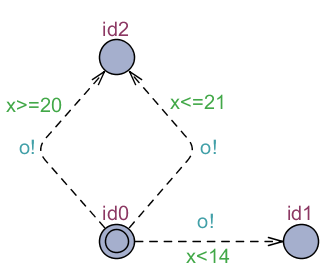
\includegraphics[scale = 0.7]{figures/determ.png}
    \caption{Non-deterministic automaton test case, which is not caught by \ecdar 0.10.}
    \label{fig:K7}
\end{figure}

\section{Consistency tests} \label{sec:consistTests}
An important part of the tests that were performed are the consistency tests. We have tried to create automata which would include the rarest corner cases. The case illustrated in Figure \ref{fig:G17}, where the consistency check starts in location \textbf{id0} satisfies the least fixpoint consistency check, but not the greatest fixpoint consistency check. It is important to remember that the least fixpoint consistency permits pruning of output edges if the property of independent progress has already been satisfied for a given location. Since the property of independent progress is satisfied already in location \textbf{id0} and there are no outgoing input edges, which are mandatory to explore, the algorithm prunes the rest of the automaton.

\begin{figure}
    \centering
    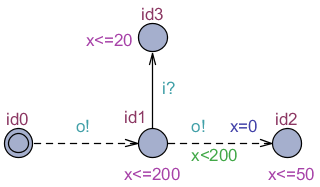
\includegraphics[scale = 0.8]{figures/test-aut-leastCons.png}
    \caption{Automaton that will only satisfy the least fixpoint consistency check.}
    \label{fig:G17}
\end{figure}

Note how the rest of the automaton does not satisfy the property of independent progress. In location \textbf{id1} the independent progress property is violated by the corresponding invariant ($x\leq200$) which disallows delaying indefinitely. Moreover, both outgoing edges from location \textbf{id1} must then be explored. Since the targets of those edges cannot ensure independent progress either, we conclude that none of the three mentioned locations would satisfy the consistency check. With that being said, this test case automaton can only satisfy the least fixpoint consistency check due to pruning of the rest of the automaton, except for location \textbf{id0}.


\section{Implementation tests}
The defining property of the implementation check is the one of the output urgency. It requires any output edge to be traversable only with a single clock valuation, without the possibility to delay instead. Consider the test case illustrated in Figure \ref{fig:G19}. This automaton is consistent and the only output edge it has is urgent, which satisfies the property of the output urgency for the entire automaton. 

Moreover, it is important to remember that the implementation check also requires a consistency check that is different from the least fixpoint consistency check mentioned previously in this chapter. Since the property of output urgency concerns all output edges, the corresponding consistency check should not be allowed to prune these edges, resulting in having to perform a full consistency check, which was described in Section \ref{sec:minConsistency}. Thus, having an invariant on location with \textbf{id2} makes the implementation check fail due to the property of independent progress not being satisfied.
\begin{figure}
    \centering
    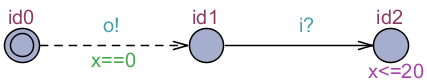
\includegraphics[scale = 0.7]{figures/G19.png}
    \caption{Automaton that fails full consistency check that is required by implementation check.}
    \label{fig:G19}
\end{figure}

\section{Summary}

To conclude the chapter, more thorough and detailed testing was done for all the existing and newly implemented features. In particular, we focused on testing all the corner cases that were discovered during this project as well as cases where \ecdar 0.10 has shown to be inconsistent with the theory.

In total there are currently more than \todo{recheck this number}320 quality tests in \jecdar, which is 170 more than in the previous version of the engine. The code coverage of the most vital functionality related to feature verification has also been improved from previously achieved more than 95 percent to a complete 100 percent coverage, as can be seen in Figure \ref{fig:code-coverage}. What is more important, in its implementation \jecdar does not contain the same inconsistencies with the theory as discovered in \ecdar 0.10.

\begin{figure}
    \centering
    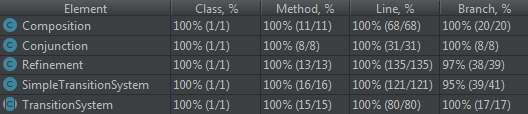
\includegraphics[scale = 0.7]{figures/code-coverage.png}
    \caption{Code and branch coverage of the most important verification algorithms.}
    \label{fig:code-coverage}
\end{figure}

In addition to the line coverage metrics, we have also considered branch coverage. It measures if all decision outcomes have been tested, where a decision can be \textit{if} and \textit{case} statements, \textit{while} and \textit{for} loops. This metrics shows if all branches (possible cases of decisions) were ever reached and consequently if the test case suite covers all possible decisions. 

The current test case suite of \jecdar achieves a minimum of 95 percent branch coverage (Figure \ref{fig:code-coverage}). The missing percentage of the branch coverage for \textit{Refinement} and \textit{SimpleTransitionSystem} classes is related to checking validity of the DBM zone, which appears to never be invalid and thus does not explore the negative outcome of an IF statement. However, such cases do not influence the correctness of the algorithms as they are validity checks that appear to never fail. Therefore we deem it not important.
\chapter{Conclusion and Future Work}

\section{Conclusion}\label{sec:conclusion}
The result of our work spanning two semesters, \jecdar, is an engine for modelling and verifying properties of real-time systems based on the specification theory of timed input/output automata defined in \textcite{David:2010}. Although there already exists an integrated environment that can do this, namely \ecdar, this tool requires a license for non-academic use. Our engine addresses this issue by being open-source and it is meant to be integrated with a GUI that allows efficient creation of models and verification of properties.

\jecdar is not a finished tool, as it lacks some of the features available in \ecdar, such as computing quotient, running models in a simulator and checking TCTL formulas. The aim of the project was to implement features that perform correctly, which meant that the goal of implementing as many features as possible was downgraded. Currently, \jecdar can be used to check features such as consistency, implementation and refinement and it can operate on the composition and conjunction of multiple transition systems.

The result of this process is not an engine that behaves exactly like \ecdar, meaning that there are several implementation differences between the two engines. A large part of our process consisted of discovering cases where \ecdar displays inconsistencies with the theory and devising ways to tackle said cases.

This report documented our initial goal for the project, observations regarding scenarios that display inconsistencies between \ecdar and the theory of timed input/output automata, concepts that we used for the purpose of correctly implementing certain features (both successful and unsuccessful), implementation details and a description of our testing approach.

\section{Future Work}\label{sec:future}
In this chapter we introduce some of prominent ideas for future work that can be conducted on \jecdar engine. Note that this chapter does not include the points from the future work described in our previous semester, which can be found in \textcite{Jecdar:2019}.

\subsection{Greatest fixpoint consistency}
Currently, \jecdar includes the least fixpoint consistency check as well as the full consistency check used in the implementation check. An interesting subject for future work can however be the computation of the greatest fixpoint consistency, described in Section \ref{sec:minConsistency}.

\subsection{Returning refinement relation}
\todo{recheck}
Even though this time the main focus was on refinement, there still exists one more possibility regarding it. Right now \jecdar is capable of returning the list of state pairs which participate in the refinement relation, however it is not being visually shown, so this gives us the future possibility of visually displaying the refinement relation.

\subsection{Support user-defined variables}
\ecdar 0.10 supports record variables, which are specified by the keyword $struct$, which follows the $C$ notation. An example of a record $k$ can be seen in Listing \ref{lst:struct}. Thus, user-defined variables can be a good candidate for new features in \jecdar.
\begin{lstlisting}[caption={Record example},label={lst:struct}, captionpos=b]
struct{
     int x;
     int y;
} k;         
\end{lstlisting}

\subsection{TCTL formulas}
Since \ecdar 0.10 is built on top of \uppaal it includes TCTL formulas, which could be a subject for improvement in \jecdar. 

\subsection{State-space reduction techniques}
The field of model-checking is known for having the problem of exponential state-space growth during its exploration.
This can be another improvement that \jecdar can benefit from - the introduction of state-space reduction techniques. Some of such techniques can greatly reduce the amount of time and memory required during state-space exploration.

As already mentioned previously our focus is on correctness rather than performance. At the moment, \jecdar is making use of a rather primitive implementation of extrapolation abstraction. Hence, a very promising potential performance improvement could include implementation of more advanced extrapolation abstraction techniques, such as location-based bounds for extrapolation or lower and upper bound dependent extrapolation. For some models with very big values of the time-progress conditions (guards and invariants) this could greatly reduce the size of the state-space that has to be explored.

Another case of abstraction could be the symmetry reduction. It is based on the \textit{state swaps} that are used to reduce the size of the state-space that has to be explored, consequently reducing time and memory needed for verification. According to \textcite{SymmetryReduction}, to achieve that a suitable bisimulation equivalence has to be derived from the system description, introducing the necessity for the engine to support such declarations. Afterwards, the representative function is constructed and used to convert a state into a corresponding equivalence class. Then when doing a reachability analysis it suffices to explore and store only one representative of equivalence class.

\printbibliography[heading=bibintoc]
\label{bib:mybiblio}
\appendix
\chapter[Refinement relation in JSON format]{Refinement relation\\ in JSON format}\label{ch:jsonRR}
\begin{lstlisting}[language=json,firstnumber=1,tabsize=2]
{
"left": "id45",
"zone": "[1, 1, 1, 2147483646, 1, 1, 2147483646, 1, 1]",
"right": "id41",
"initial sp id": "0",
"transitions": [{
		"source sp id": "0",
		"channel": "ro",
		"target sp id": "1",
		"target sp": {
			"left": "id44",
			"zone": "[1, 1, 1, 13, 1, 1, 13, 1, 1]",
			"state pair id": "1",
			"right": "id40",
			"transitions": [{
					"source sp id": "1",
					"channel": "go",
					"target sp id": "2",
					"target sp": {
						"left": "id42",
						"zone": "[1, 1, 1, 13, 1, 1, 13, 1, 1]",
						"state pair id": "2",
						"right": "id40",
						"transitions": [{
								"source sp id": "2",
								"channel": "ri",
								"target sp id": "4",
								"target sp": {
									"left": "id43",
									"zone": "[1, 1, 1, 2147483646, 1, 1, 2147483646, 1, 1]",
									"state pair id": "4",
									"right": "id39"
								}
							}
						]
					}
				}, {
					"source sp id": "1",
					"channel": "ri",
					"target sp id": "3",
					"target sp": {
						"left": "id44",
						"zone": "[1, 1, 1, 13, 1, 1, 13, 1, 1]",
						"state pair id": "3",
						"right": "id39",
						"transitions": [{
								"source sp id": "3",
								"channel": "go",
								"target sp id": "5",
								"target sp": {
									"left": "id42",
									"zone": "[1, 1, 1, 13, 1, 1, 13, 1, 1]",
									"state pair id": "5",
									"right": "id39",
									"transitions": [{
											"source sp id": "5",
											"channel": "ri",
											"target sp id": "4"
										}
									]
								}
							}
						]
					}
				}
			]}}]}



\end{lstlisting}
\end{document}